
\documentclass[12pt,singleside,a4paper]{article}

\usepackage[utf8]{inputenc}
\usepackage{mwe}
\usepackage{graphicx}
\usepackage{epsfig}
\usepackage{cite}
\usepackage{geometry}
\usepackage{float}
\usepackage{subfig}
\usepackage{comment}
\usepackage{listings}
\usepackage{minted}
\usepackage[usenames,dvipsnames]{xcolor}


\definecolor{vgreen}{RGB}{104,180,104}
\definecolor{vblue}{RGB}{49,49,255}
\definecolor{vorange}{RGB}{255,143,102}


\lstdefinestyle{verilog-style}
{
    language=Verilog,
    frame=single,
    linewidth=18cm,
    basicstyle=\small\ttfamily,
    keywordstyle=\color{vblue},
    identifierstyle=\color{black},
    commentstyle=\color{vgreen},
    moredelim=*[s][\colorIndex]{[}{]},
    literate=*{:}{:}1
}

%%%%%%%%%%%%%%%%%vhdl%%%%%%%%%%%%%%%%%%%%

\lstdefinelanguage{VHDL}{
   morekeywords=[1]{
     LIBRARY,USE,ENTITY,IS,PORT,IN,OUT,END,ARCHITECTURE,OF,
     BEGIN,DOWNTO,ALL,WAIT,FOR,OTHERS,SIGNAL,PROCESS
   },
   morekeywords=[2]{
     STD_LOGIC_VECTOR,STD_LOGIC,IEEE,STD_LOGIC_1164,
     NUMERIC_STD,STD_LOGIC_ARITH,STD_LOGIC_UNSIGNED,std_logic_vector,AND,OR,NOT,NAND,NOR,XOR,
     std_logic
   },
   morecomment=[l]--
}
\colorlet{keyword}{blue!100!black!80}
\colorlet{STD}{Lavender}
\colorlet{comment}{green!80!black!90}
\lstdefinestyle{vhdl}{
   language     = VHDL,
   basicstyle   = \footnotesize \ttfamily,
   keywordstyle = [1]\color{keyword}\bfseries,
   keywordstyle = [2]\color{STD}\bfseries,
   commentstyle = \color{comment}
}
%%%%%%%%%%%%%%%%%%%%%%%%%%%%%%%%%%%%%%%%%%%%%%%%%%%

\geometry{left=20mm,right=20mm,top=20mm,bottom=40mm}


\begin{document} 

\begin{titlepage}
	\centering
    \textsc{\LARGE 2-Bit Ripple Adder}\\[2.0 cm]
\begin{figure}[!htb]
\centering
  
\includegraphics[width=3cm,keepaspectratio]{logo.png}\textbf{ }\textbf{  }
  
\includegraphics[width=3cm,keepaspectratio]{download.png}\textbf{  }
  
\includegraphics[width=3cm,keepaspectratio]{modelsim-logo.jpg}
\end{figure}	\\[2cm]\
	\begin{minipage}{0.4\textwidth}
		\begin{flushleft} \large
			\emph{Mentors}\\
			Prasad T\\
            Aditya Gudla\\
            Simranjeet Singh \
			\end{flushleft}
			\end{minipage}~
			\begin{minipage}{0.4\textwidth}
            
			\begin{flushright} \large
			\emph{Interns} \\
			Ajay Chaudhari\\
            Chethan T Bhat\\
            Ritvik Tiwari \\
            Karthik A Shet \\
		\end{flushright}
	\end{minipage}\\[2 cm]
\end{titlepage}
\pagenumbering{arabic}
\newpage
\tableofcontents
\newpage
\pagenumbering{arabic}
\section{Introduction}
Full Adder is an adder which adds three inputs and produces two outputs. The first two inputs are A and B and the third input is an input carry, C-IN. The output carry is designated as C-OUT and the Sum output is designated as S.
\newline
\newline
Multiple full adder circuits can be cascaded in parallel to add an N-bit number. For an N- bit parallel adder, there must be N number of full adder circuits. A ripple carry adder is a logic circuit in which the carry-out of each full adder is the carry in of the succeeding next most significant full adder. It is called a ripple carry adder because each carry bit gets rippled into the next  stage. We obtain an output carry (C-OUT) and an N- bit sum (S).
\newline
\newline
For this project we will be using the full adder design for our 2-bit ripple carry adder
\begin{figure}[H]
    \centering
    
\includegraphics[scale=0.4]{circuit_diagram.png}
    \caption{Full Adder}
\end{figure}

\begin{figure}[H]
    \centering
    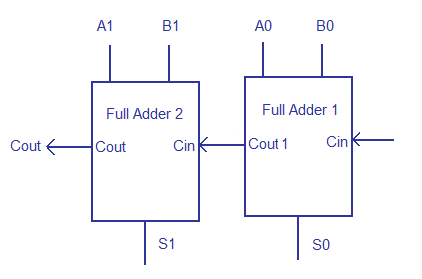
\includegraphics[scale=0.8]{ripple.png}
    \caption{2-bit Ripple Carry Adder}
\end{figure}

\begin{center}
\begin{tabular}{ |p{1cm}|p{1cm}|p{1cm}|p{1cm}|p{1cm}|  } \hline
 \multicolumn{5}{|c|}{Truth Table for Full Adder}   \\ \hline \hline
    A   &   B   &  Cin  &  Sum  &   Carry           \\ \hline
    0   &   0   &   0   &   0   &   0               \\\hline
    0   &   0   &   1   &   1   &   0               \\\hline
    0   &   1   &   0   &   1   &   0               \\\hline
    0   &   1   &   1   &   0   &   1               \\\hline
    1   &   0   &   0   &   1   &   0               \\\hline
    1   &   0   &   1   &   0   &   1               \\\hline
    1   &   1   &   0   &   0   &   1               \\\hline
    1   &   1   &   1   &   1   &   1               \\\hline

\end{tabular} 
\captionof{table}{Truth Table for Full Adder}
\end{center}




\section{VHDL Codes}
\subsection{Code for Full Adder Dataflow Modelling:}
\begin{lstlisting}[style=VHDL, frame=single,linewidth = 18cm]
--Full Adder VHDL Code
--Including Libraries
LIBRARY IEEE;
USE 	IEEE.STD_LOGIC_1164.ALL;
USE 	IEEE.NUMERIC_STD.ALL;

--Full Adder Entity Declaration
ENTITY full_adder IS
	PORT(
		A 	: IN 	STD_LOGIC;  --Input A
		B 	: IN 	STD_LOGIC;  --Input B
		CIN	: IN 	STD_LOGIC;  --Input CIN			
		Sum : OUT STD_LOGIC;    --Output SUM
		COUT: OUT STD_LOGIC     --Output CARRY
		);
	END  full_adder;
	
--Architecture Declaration	
ARCHITECTURE BEHAVIOURAL OF full_adder IS
	--Main Logic
	BEGIN
		
		Sum   <=  A XOR B XOR CIN;
		COUT<= (A AND B) OR (CIN AND (A XOR B));
			
END BEHAVIOURAL;

\end{lstlisting}

\newpage

\subsection{Code for 2 Bit Ripple Carry Full Adder}
\begin{lstlisting}[style=VHDL, frame=single,linewidth = 18cm]
--We have incorporated the full adder entity from the previous 
--code for the 2 bit ripple carry full adder

LIBRARY 	IEEE;
USE 		IEEE.STD_LOGIC_1164.ALL;
USE 		IEEE.NUMERIC_STD.ALL;

--Ripple Carry Adder Entity 
ENTITY ripple_carry_adder IS
  PORT(
	  A: IN STD_LOGIC_VECTOR (1 DOWNTO 0); --2 bit Vector input A
	  B: IN STD_LOGIC_VECTOR (1 DOWNTO 0); --2 bit Vector input B
	  CIN: IN STD_LOGIC;
	  Sum: OUT STD_LOGIC_VECTOR (1 DOWNTO 0);--2 bit Vector output SUM
	  COUT: OUT STD_LOGIC
	  );
			
END ENTITY ripple_carry_adder;
 
 --Architecture Declaration
ARCHITECTURE BEHAVIOURAL OF ripple_carry_adder IS
	COMPONENT full_adder
		PORT(
			A 	: IN 	STD_LOGIC;
			B 	: IN 	STD_LOGIC;
			CIN	: IN 	STD_LOGIC;
			Sum : OUT STD_LOGIC;
			COUT : OUT STD_LOGIC
			);
				  END COMPONENT;
 
		SIGNAL C1	: STD_LOGIC;
		--Main Architecture
		--We have used the previously designed full_adder modules here
		BEGIN
			--Over here we have used PORT MAP for mapping the current 
			--inputs with the full_adder module
			FA0: full_adder PORT MAP( A(0),B(0),CIN,Sum(0), C1 );
			FA1: full_adder PORT MAP( A(1),B(1), C1,Sum(1), COUT);
 
END BEHAVIOURAL;

\end{lstlisting}

\newpage
\subsection{Test Bench for Ripple Carry Adder}
\begin{lstlisting}[style=VHDL, frame=single,linewidth = 18cm]
--VHDL Test Bench

--Including Libraries
LIBRARY ieee;
USE ieee.std_logic_1164.ALL;
 
--Entity Declaration
 ENTITY tb_ripple_carry_adder IS
END tb_ripple_carry_adder;
 
 
--Architecture Declaration
ARCHITECTURE behavior OF tb_ripple_carry_adder IS
 
-- Component Declaration for the Unit Under Test (UUT)
 
COMPONENT ripple_carry_adder
PORT(
A : IN STD_LOGIC_VECTOR(1 DOWNTO 0);
B : IN STD_LOGIC_VECTOR(1 DOWNTO 0);
CIN : IN STD_LOGIC;
Sum : OUT STD_LOGIC_VECTOR(1 DOWNTO 0);
COUT : OUT STD_LOGIC
);
END COMPONENT;
 
--Inputs
SIGNAL A : STD_LOGIC_VECTOR(1 DOWNTO 0) := (OTHERS => '0');
SIGNAL B : STD_LOGIC_VECTOR(1 DOWNTO 0) := (OTHERS => '0');
SIGNAL CIN : STD_LOGIC := '0';
 
--Outputs
SIGNAL Sum : STD_LOGIC_VECTOR(1 DOWNTO 0);
SIGNAL COUT : STD_LOGIC;
 
BEGIN
 
-- Instantiate the Unit Under Test (UUT)
uut: ripple_carry_adder PORT MAP (
A => A,
B => B,
CIN => CIN,
Sum => Sum,
COUT => COUT
);
 
-- Stimulus process
stim_proc: PROCESS
BEGIN
-- hold reset state for 100 ns.
WAIT FOR 100 ns;


\end{lstlisting}\\\newpage
\begin{lstlisting}[style=VHDL, frame=single,linewidth = 18cm]
--Different combinations of two bit inputs which are fed to the adder
A <= "01";
B <= "11";
 
WAIT FOR 100 ns;
A <= "11";
B <= "11";
CIN <= '1';

WAIT FOR 100 ns;
A <= "10";
B <= "01";
 
WAIT FOR 100 ns;
A <= "00";
B <= "11";
 
 
WAIT;
 
END PROCESS;
 
END;
\end{lstlisting}

\section{Verilog Codes}
You can perform the same experiment using \textbf{VERILOG} language.
Please refer the codes given below.

\subsection{RTL Description - Full Adder}
\begin{lstlisting}[style=verilog-style]
// Verilog code for Full Adder
// Define Full Adder module
module Full_adder(
input a,b,c_in ,            // Define input ports a, b and c_in  
output sum,c_out );           // Define output ports sum and c_out
	
assign  sum    = a ^ b ^ c_in;                 // Define Sum logic
assign c_out = ((a & b)| (c_in & (a ^ b))); // Define Carry_out logic
	
endmodule	
\end{lstlisting}
\newpage
\subsection{RTL Description - Ripple Carry Adder}
\begin{lstlisting}[style=verilog-style]
// Verilog code for 2 bit ripple_carry_adder
// Define module

module Ripple_Carry_Adder(
	
	
input [1:0]a,b,
input cin,               //Define all input ports
output [1:0]Sum,
output C_Out);            // Define all ouput ports
	 
wire c1;		//Define intermediate carry as c1
	
	
Full_adder FA0(a[0],b[0],cin,Sum[0],c1); // instantiate full_adder (FA0)
Full_adder FA1(a[1],b[1],c1,Sum[1],C_Out);// instantiate full_adder (FA1)
	
	
endmodule	 		// end of module
\end{lstlisting}

\subsection{Testbench}
\begin{lstlisting}[style=verilog-style]
// Verilog code for Test bench
//Define module

module Ripple_Carry_Adder_tb;

reg [1:0]a;                     //Define all I/O ports 
reg [1:0]b;
reg cin;
wire [1:0]Sum;
wire C_Out;
	
// Map all th I/O ports with DUT
Ripple_Carry_Adder uut(.a(a) , .b(b), .cin(cin), .Sum(Sum), .C_Out(C_Out));
	
initial begin //Initialize the pins with different combination of inputs.
	
	a=2'b01; b=2'b11;  cin =1'b1;  # 100;
	a =2'b11; b=2'b11; cin =1'b1;  # 100;
	a =2'b10; b=2'b01; cin =1'b0;  # 100;
	a =2'b00; b=2'b11; cin =1'b0;  # 100;
	
	end                         // End of initial block
endmodule                      // End of module
\end{lstlisting}

\newpage
\section{Implementing on Quartus Prime}
 
Follow the below steps : 

\begin{enumerate}
    \item Start a \textbf{New Project} in Quartus Lite software
    \begin{figure}[H]
    \centering
    
\includegraphics[width=14cm,keepaspectratio]{img1.png}
    \caption{Creating New Project}
    \end{figure}
    
    \newpage
    \item You will see this screen after completing all steps. For detailed steps refer the \textbf{'Quick Start Guide to Quartus and ModelSim Software'} document.
    \newline
    \textbf{Note:} We will be using DE0 Nano Board (Cyclone IV Family EP4CE22F17C6) for entire project.
    \begin{figure}[H]
    \centering
    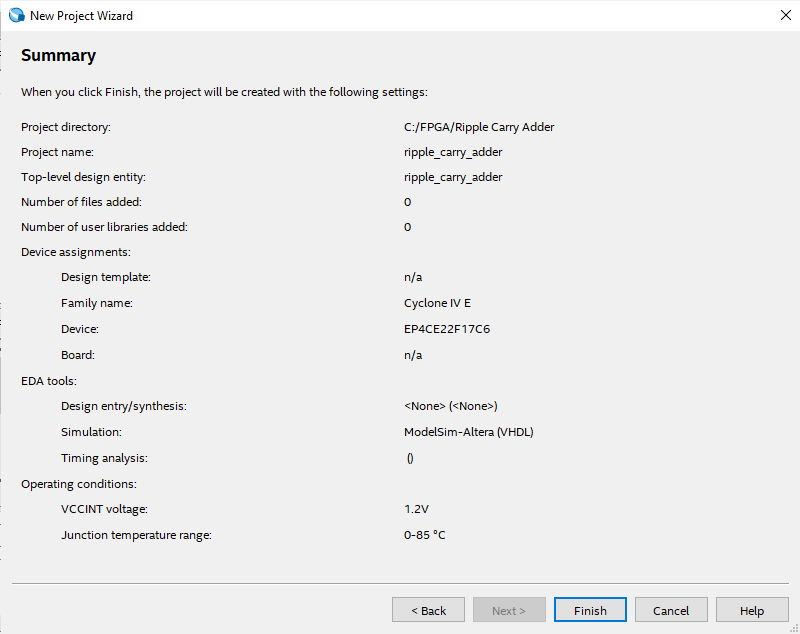
\includegraphics[width=14cm,keepaspectratio]{img2.png}
    \caption{Summary}
    \end{figure}
    
    \item We will be using \textbf{VHDL} Code throughout this project. Create a \textbf{New VHDL file}.
    \begin{figure}[H]
        \centering
    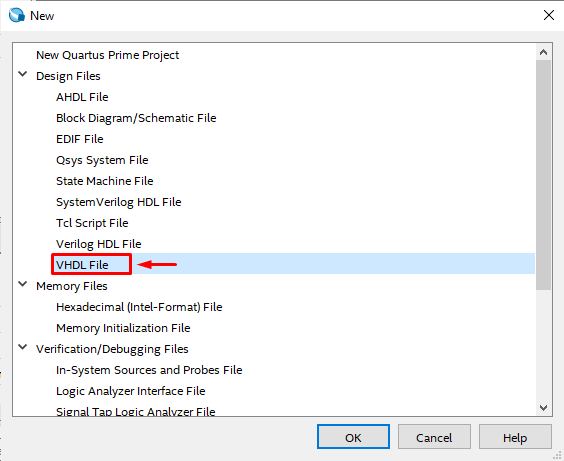
\includegraphics[width=8cm,keepaspectratio]{img3.png}
    \caption{New VHDL File}
    \end{figure}
    \newpage
    \item Type the code for full adder(code on page 2) in this file.
    \begin{figure}[H]
        \centering
    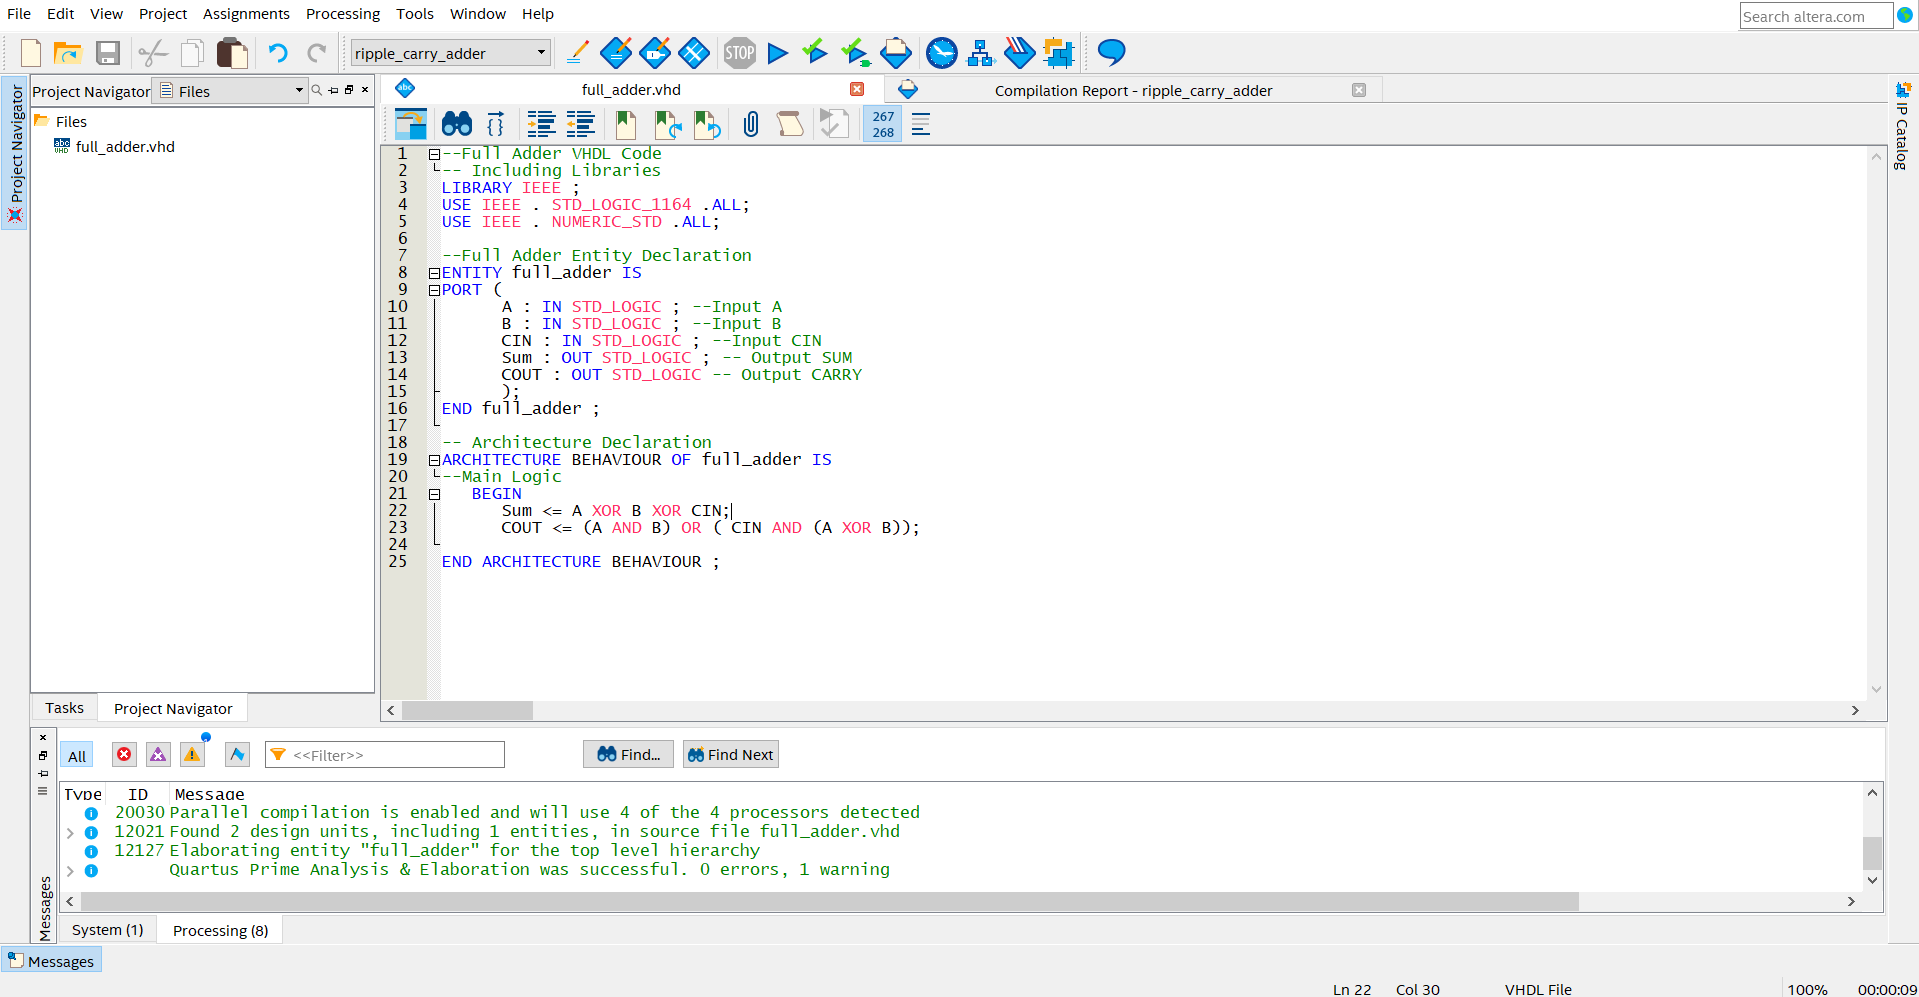
\includegraphics[width=14cm,keepaspectratio]{img3_1.png}
    \caption{VHDL Code:Full Adder}
    \end{figure}
    
    \item Go to \textbf{File}$\rightarrow$\textbf{Save as} and save the file.\textbf{Note:} File name should be same as entity name.
    \begin{figure}[H]
        \centering
    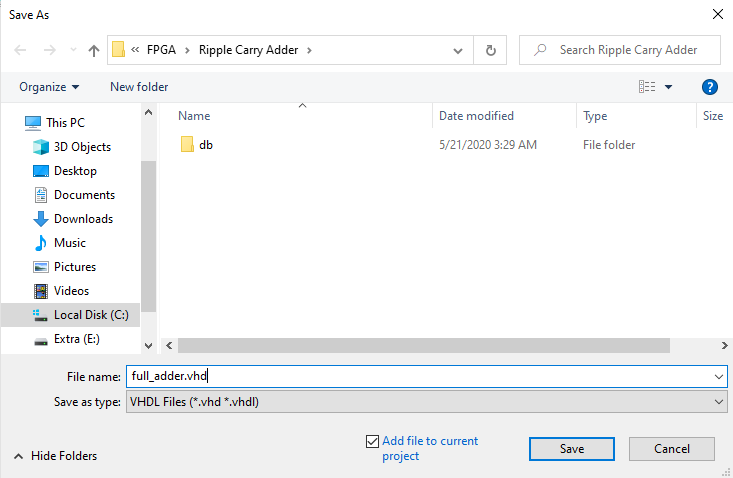
\includegraphics[width=14cm,keepaspectratio]{img4.png}
    \caption{Saving the file}
    \end{figure}
    \newpage
    \item Now, Create a \textbf{New VHDL file} again and type the code for 2-bit Ripple Carry Adder(code on page 3) in this file.
    \begin{figure}[H]
        \centering
    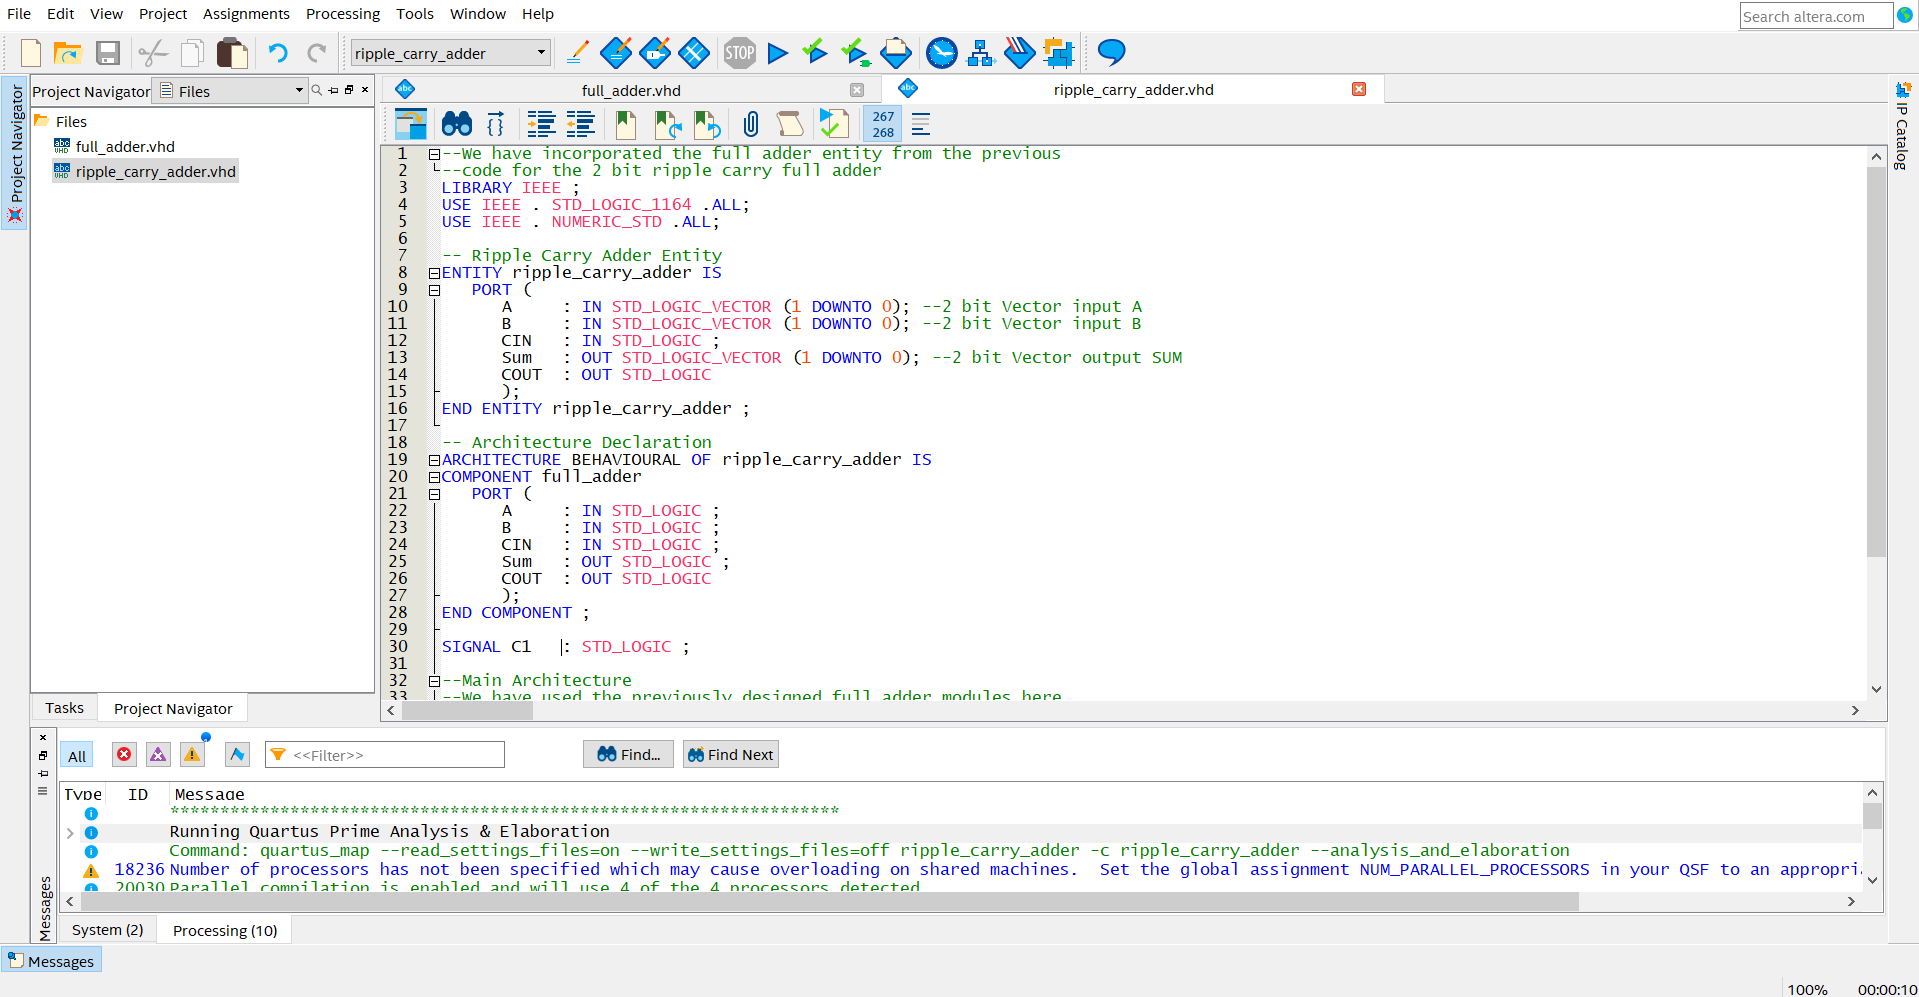
\includegraphics[width=14cm,keepaspectratio]{img4_1.png}
    \caption{|VHDL Code: 2-bit Ripple Carry Adder}
    \end{figure}
    
     \item Go to \textbf{File}$\rightarrow$\textbf{Save as} and save the file.
    \begin{figure}[H]
        \centering
    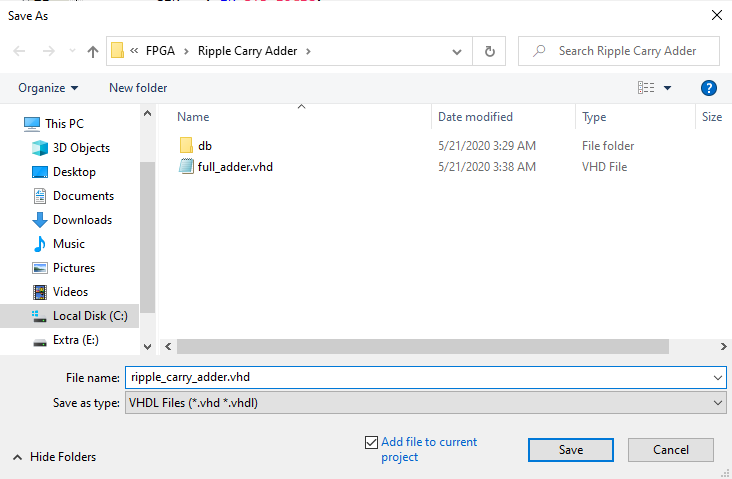
\includegraphics[width=14cm,keepaspectratio]{img5.png}
    \caption{Saving the file}
    \end{figure}
    \newpage
    \item Goto \textbf{Project}$\rightarrow$\textbf{Set as Top-Level Entity}. The \textbf{ripple\_carry\_adder} file is our main file and make sure you have selected this file while setting the top level entity.
    \begin{figure}[H]
        \centering
    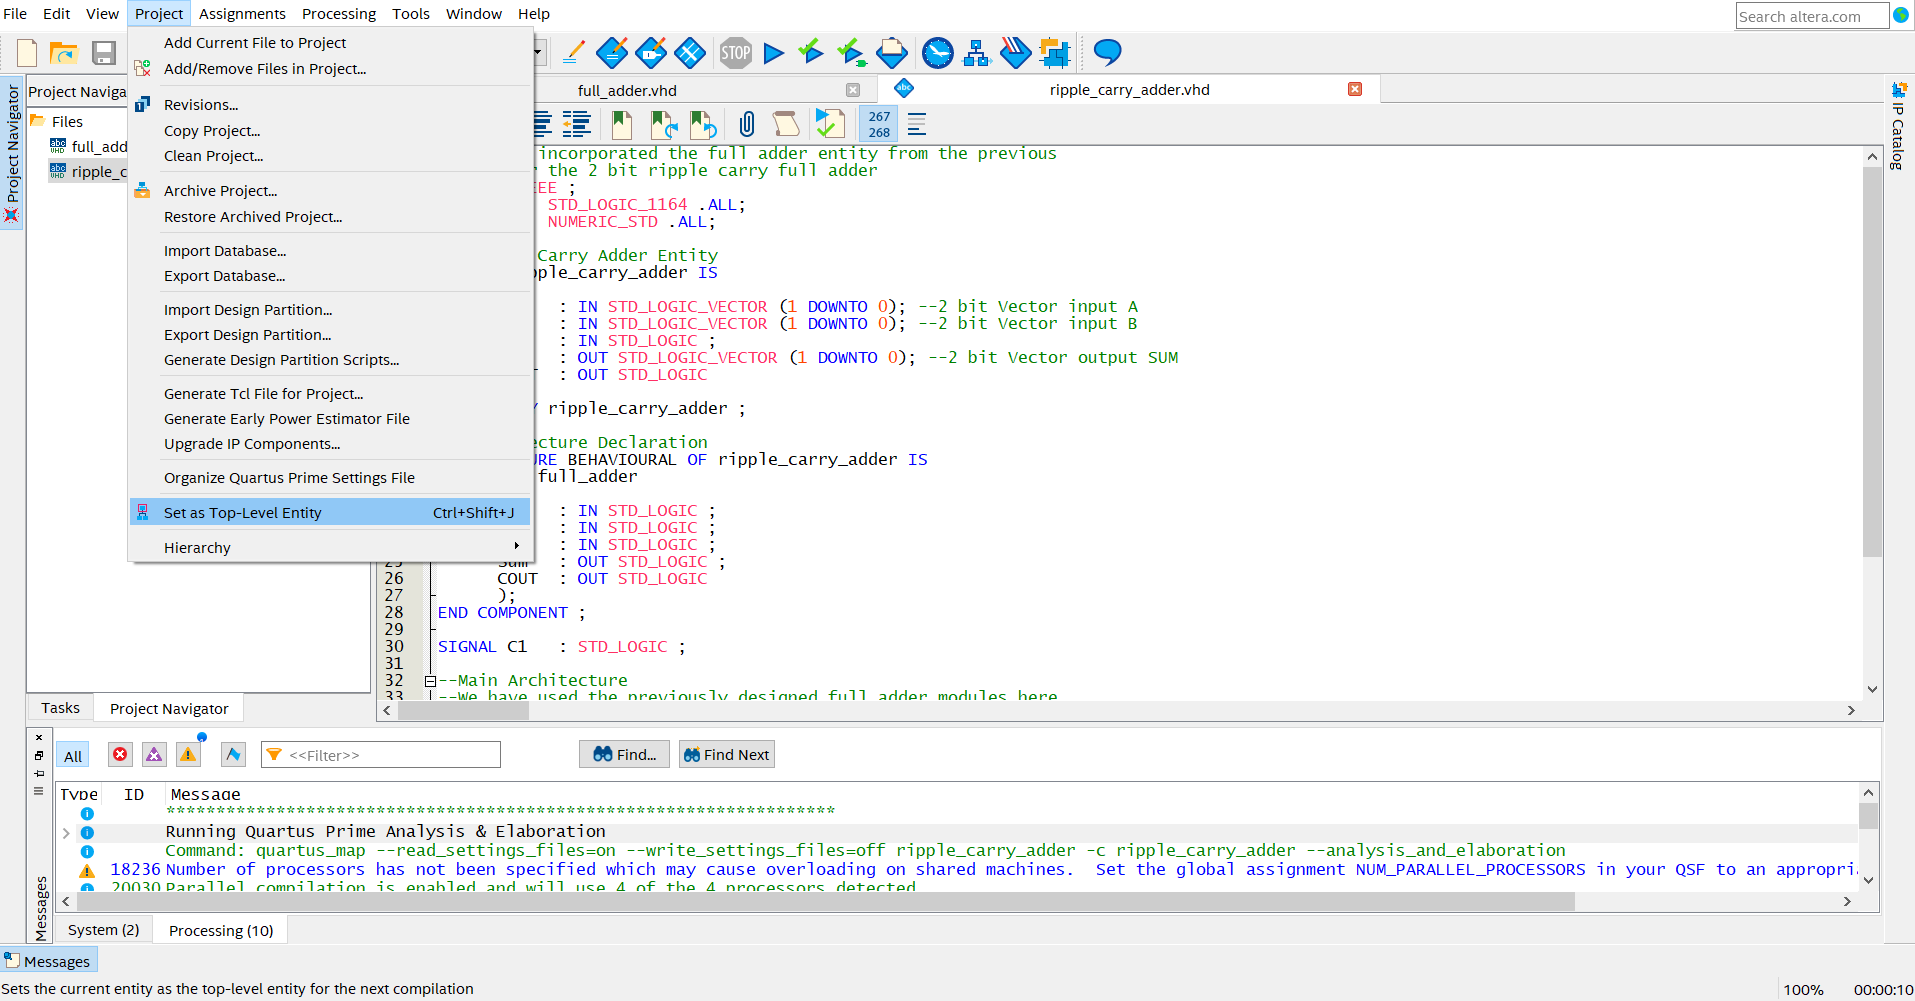
\includegraphics[width=14cm,keepaspectratio]{img6.png}
    \caption{Setting Top level entity}
    \end{figure}
    
    \item Goto \textbf{Processing}$\rightarrow$\textbf{Start Compilation}.
    \begin{figure}[H]
        \centering
    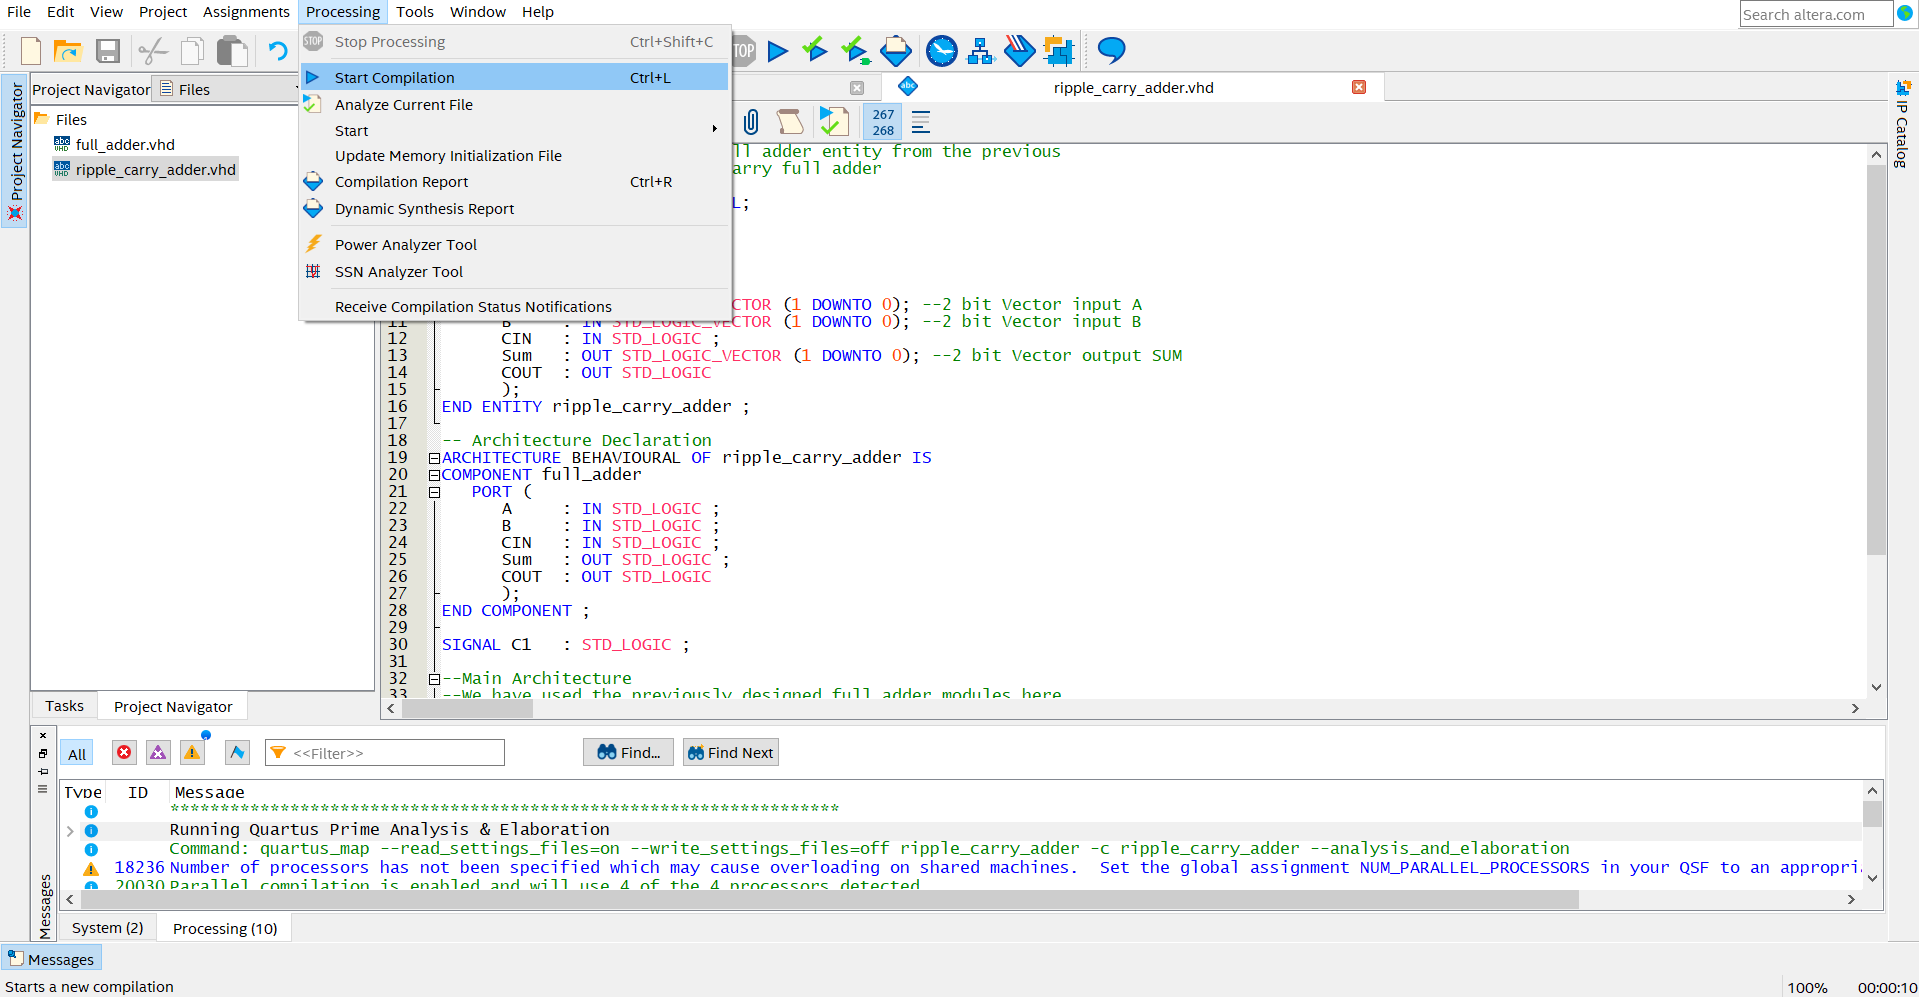
\includegraphics[width=14cm,keepaspectratio]{img7.png}
    \caption{Compiling the Design}
    \end{figure}
    \newpage
    \item You can verify whether all the files are compiled successfully by checking the highlighted tabs i.e. \textbf{Messages} and \textbf{Tasks} tab.
    \begin{figure}[H]
        \centering
    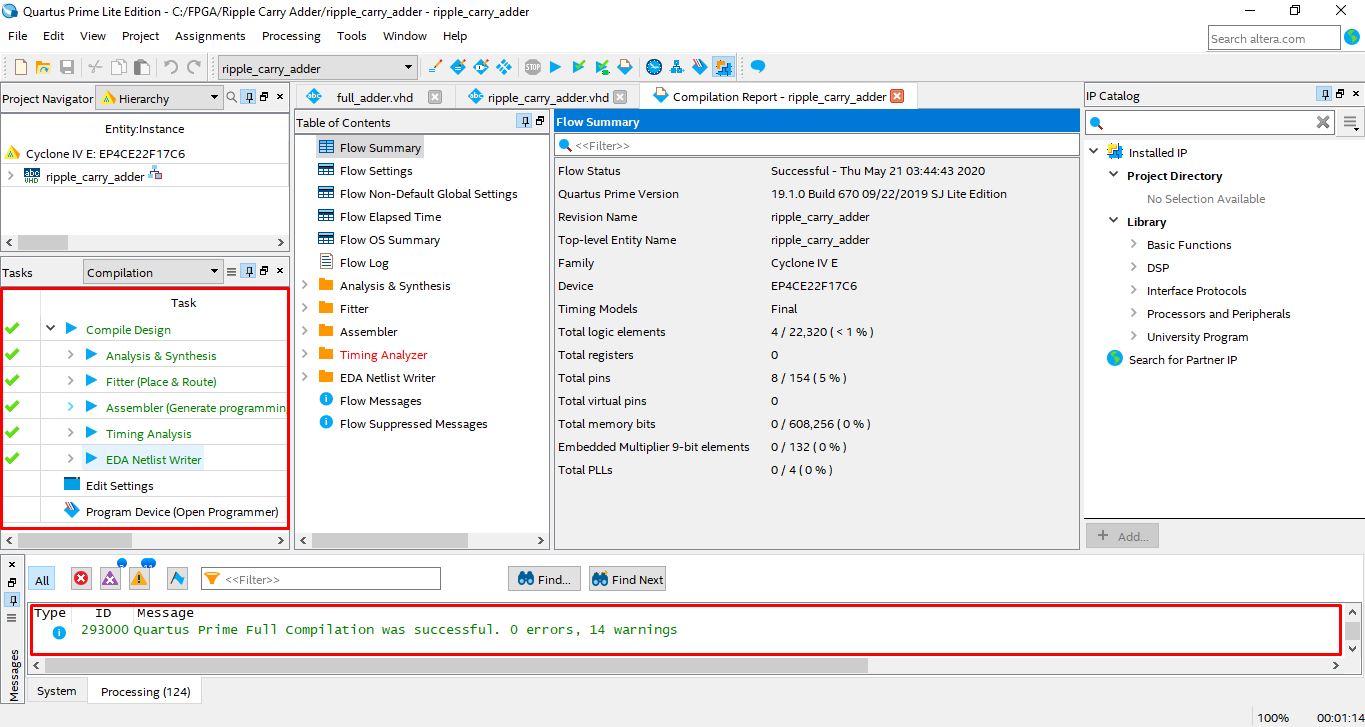
\includegraphics[width=14cm,keepaspectratio]{img8.png}
    \caption{Verification(Flow Summary)}
    \end{figure}
    
\end{enumerate}
\newpage
\section{RTL Circuit of the implemented design}
The Figure shown in step 2 below shows the RTL design of the ripple carry adder circuit. Here you can see 2 full adder modules are used. The design for these modules is incorporated from the full\_adder file.
    \subsubsection*{Steps to get RTL circuit.}
    \vspace{4mm}
        \begin{enumerate}
            \item Goto \textbf{Tools}$\rightarrow$\textbf{Netlist Viewers}$\rightarrow$\textbf{RTL Viewer}.
            \vspace{6mm}
                \begin{figure}[H]
                     \centering
                  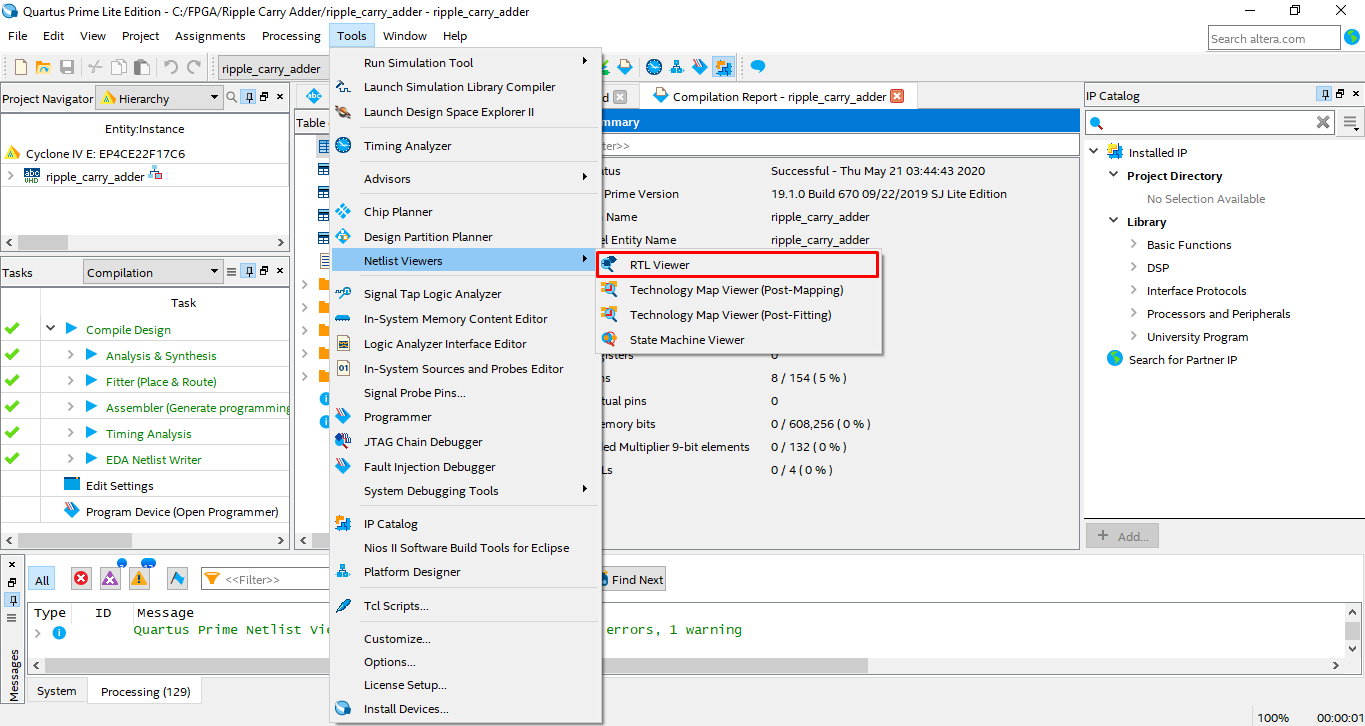
\includegraphics[width=14cm,keepaspectratio]{img9.png}
                \caption{RTL Viewer}
                \end{figure}
                \newpage
            \item The below figure shows the equivalent RTL circuit of full adder.      
\begin{figure}[H]
    \centering
    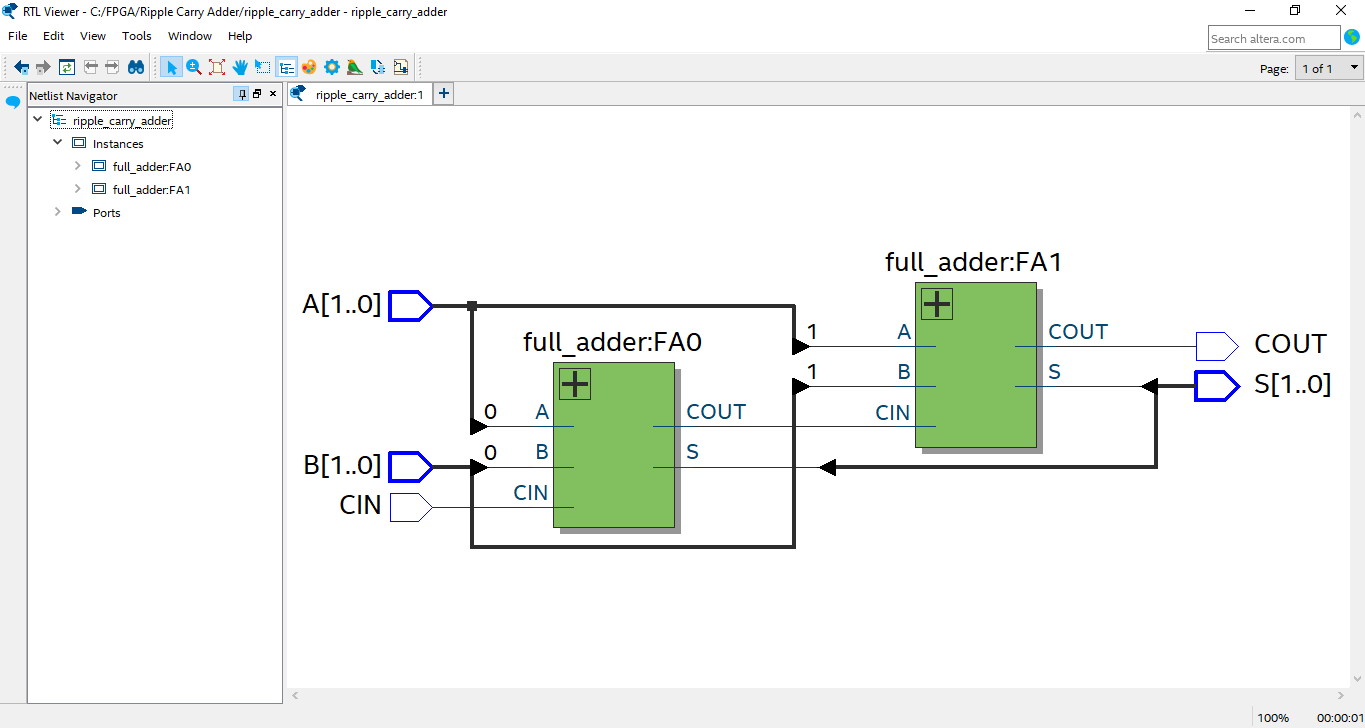
\includegraphics[width=14cm,keepaspectratio]{img10.png}
    \caption{RTL Design for 2-bit Ripple Carry Adder}
\end{figure}
\end{enumerate}

\section{Pin  Assignment}
\begin{enumerate}

    \item Click on \textbf{Assignments}$\rightarrow$\textbf{Pin Planner},This Pin Planner shows the I/O ports that we have created in our design.
    \begin{figure}[H]
        \centering
        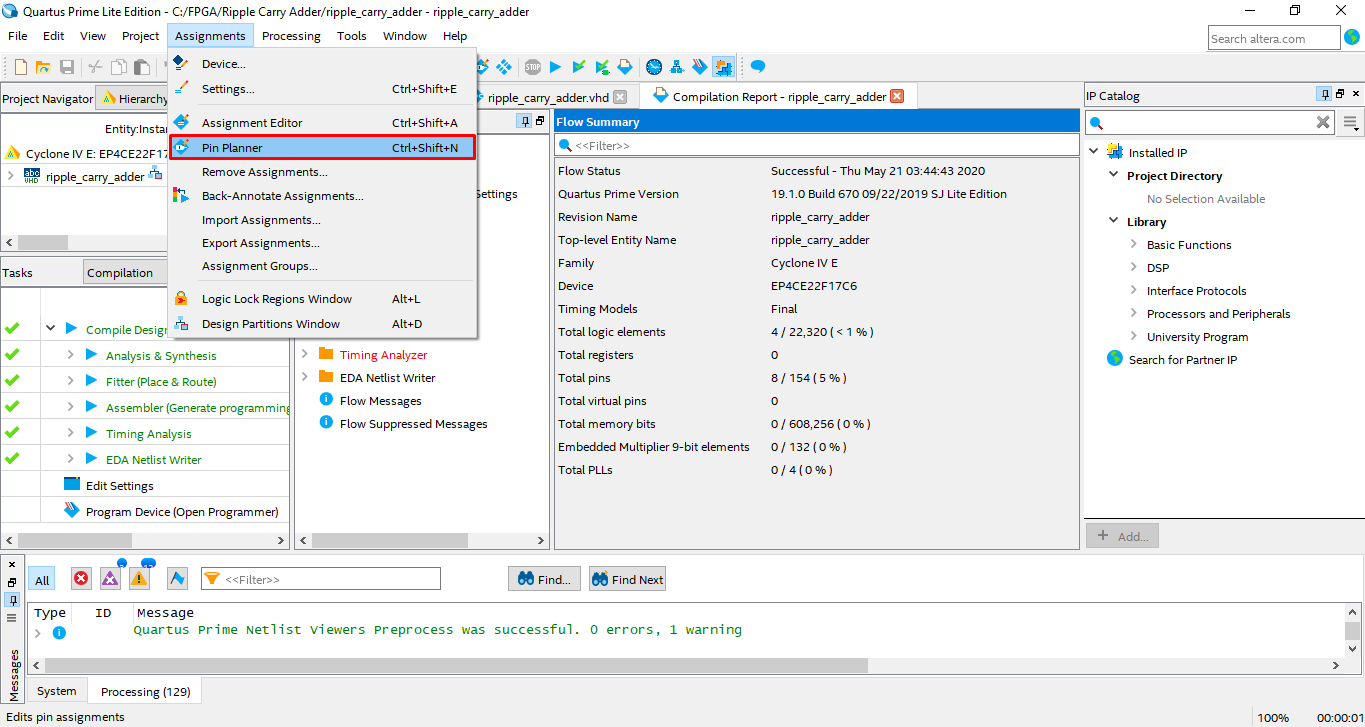
\includegraphics[width=14cm,keepaspectratio]{img11.png}
    \caption{Pin Planner}
    \end{figure}
    \newpage
    \item We will now assign the pins for Input and Output in the Location tab present in the highlighted window.
    \begin{figure}[H]
        \centering
        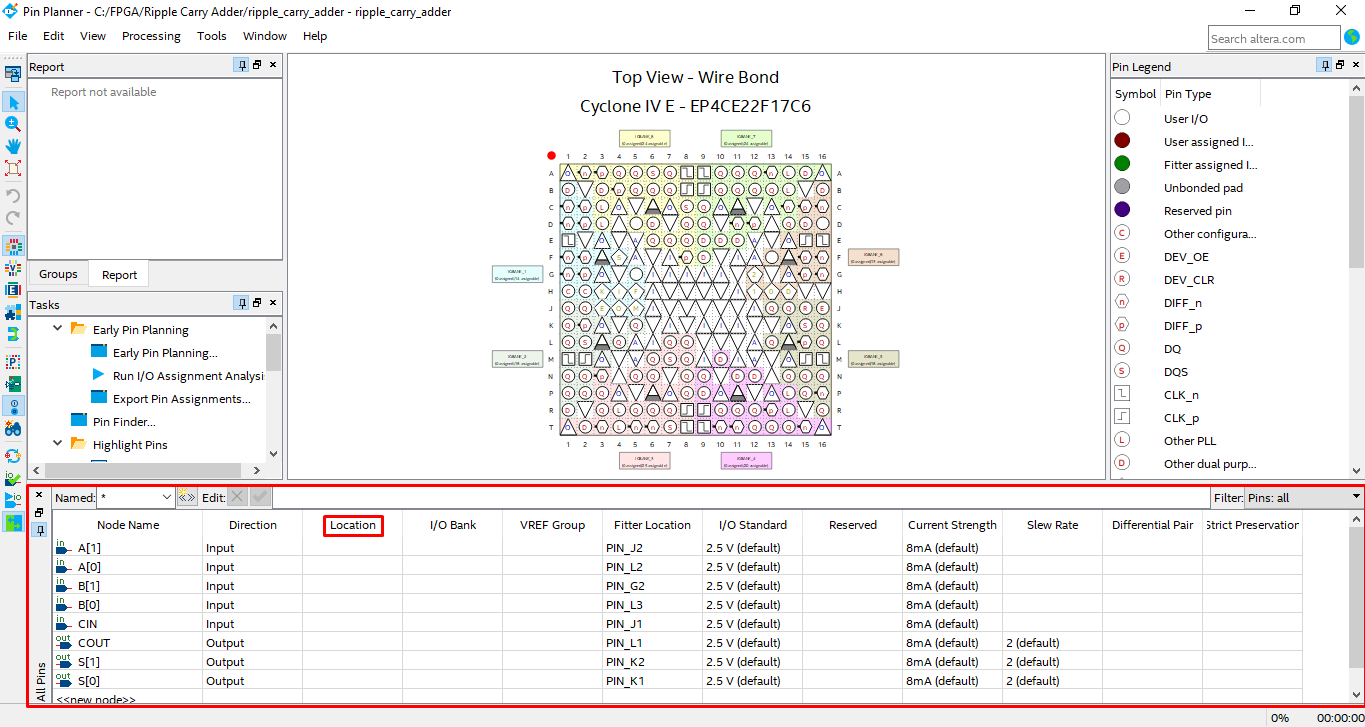
\includegraphics[width=14cm,keepaspectratio]{img12.png}
    \caption{Assigning Pins}
    \end{figure}
    
    \item Now we have to assign each I/O ports with the respective Pin numbers, which can be found in the Device Manual of the FPGA Board.Here we are referring to the DEO NANO Board . We have demonstrated how to assign the DIP[0] switch to the first input(A[1]) in the following image. You can assign all the other \textbf{Inputs} and \textbf{Outputs} in similar manner.
    
     \begin{figure}[H]
        \centering
        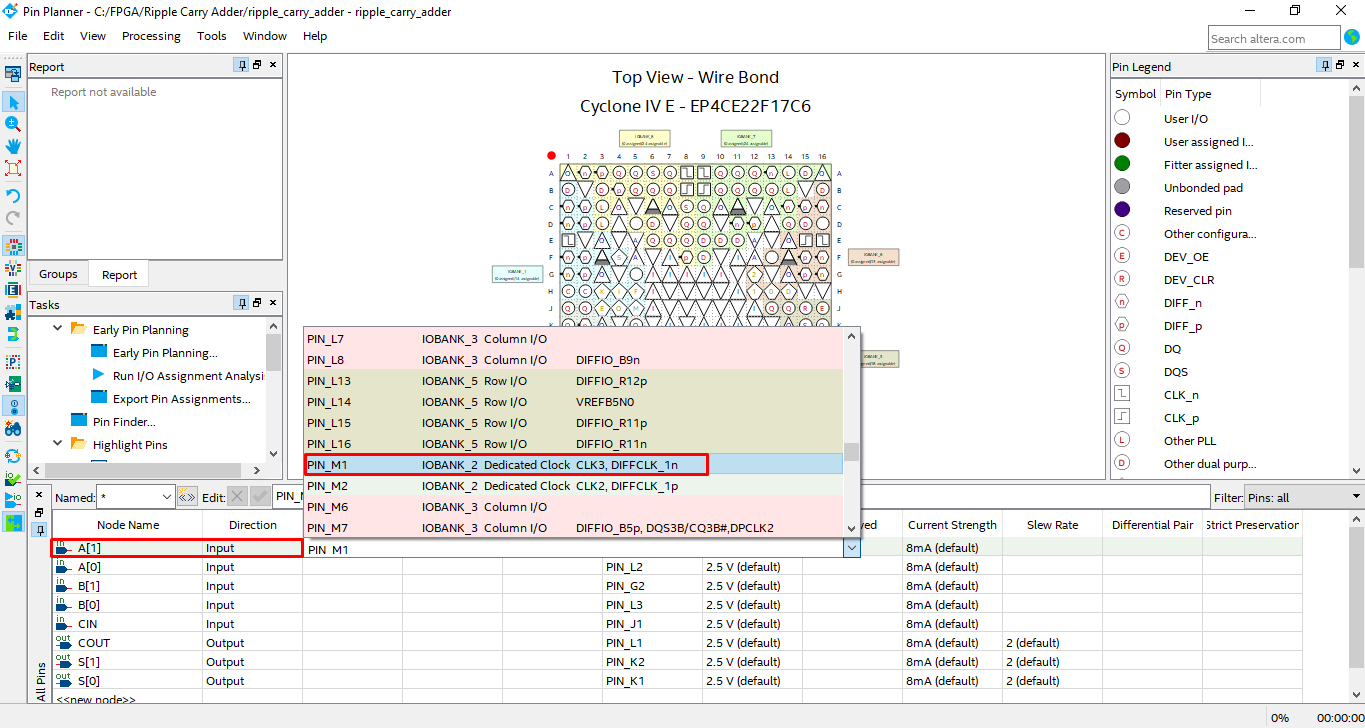
\includegraphics[width=14cm,keepaspectratio]{img13.png}
    \caption{Assigning Pins}
    \end{figure}
    \newpage
    \item After assigning all the pins your window would be similar to the following image. You can verify the pin assignments from the following image.
    \begin{figure}[H]
        \centering
        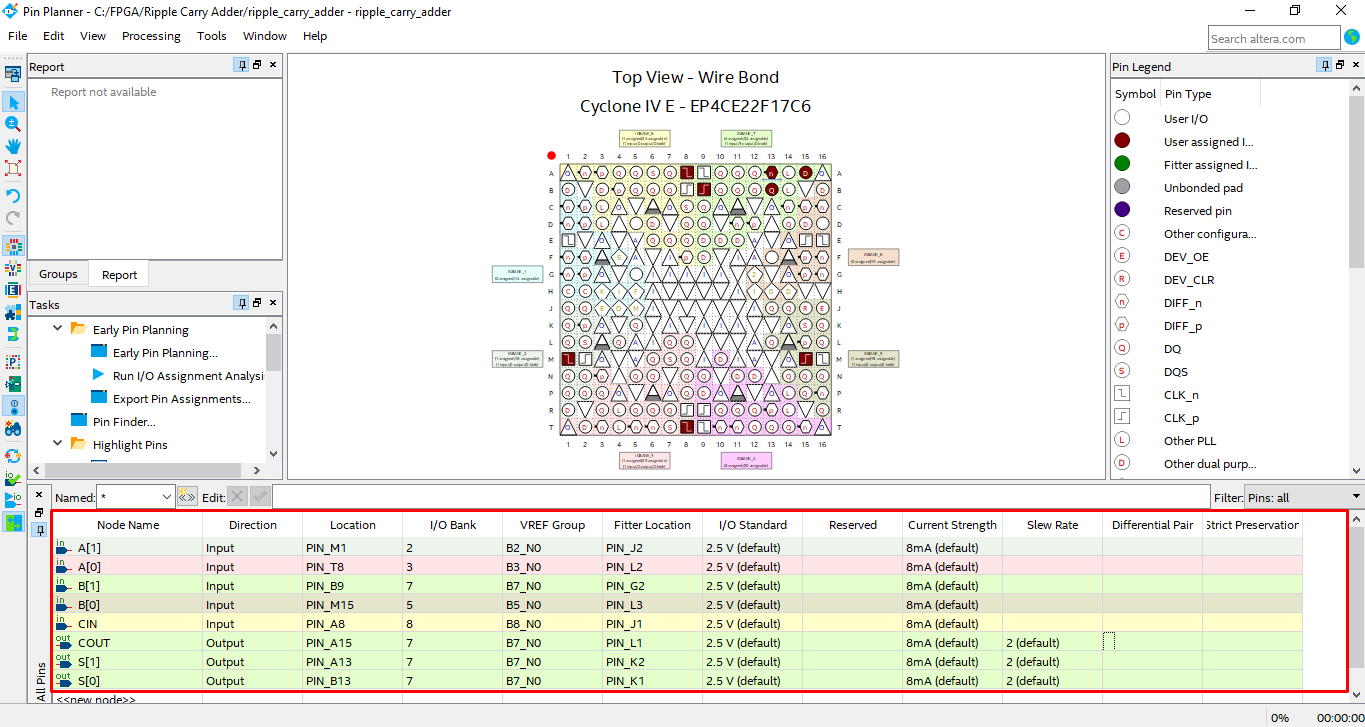
\includegraphics[width=14cm,keepaspectratio]{img14.png}
    \caption{Verifying Pin Assignment}
    \end{figure}
    
    \item Go to \textbf{Processing}$\rightarrow$\textbf{Start I/O Assignment Analysis}.
        \begin{figure}[H]
             \centering
            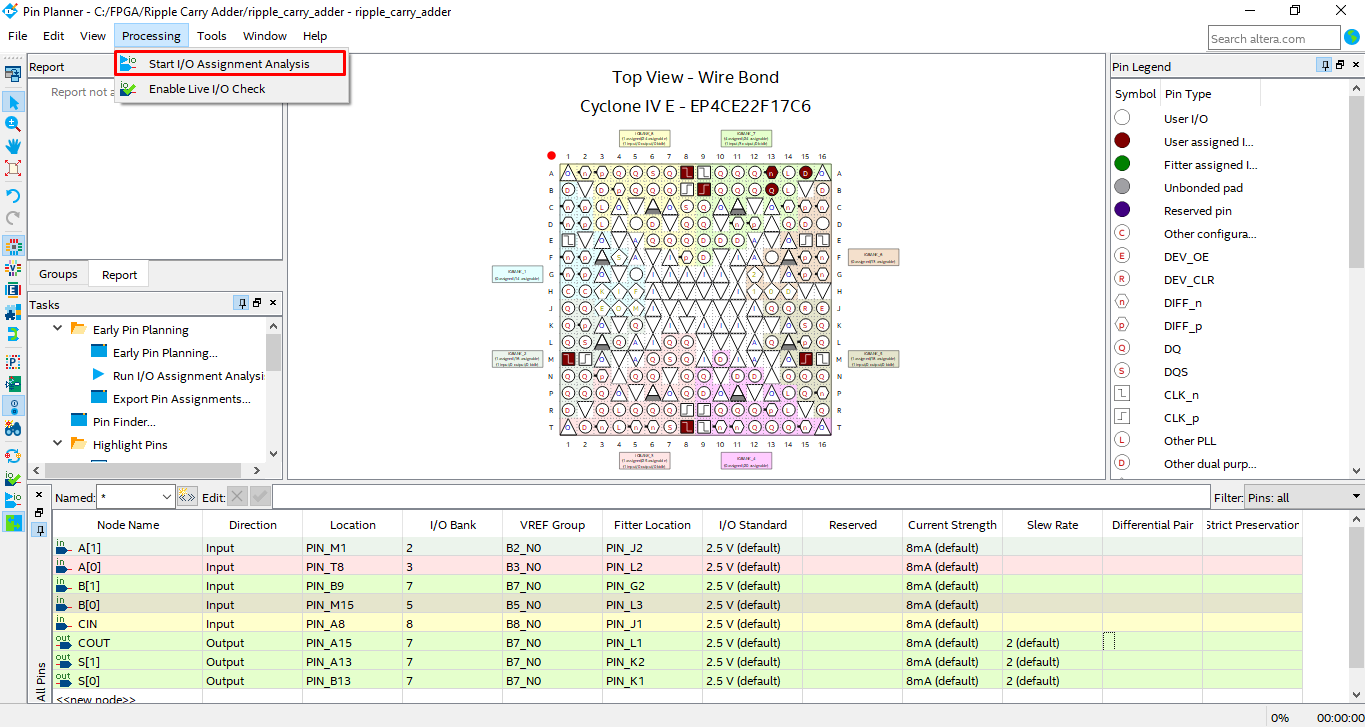
\includegraphics[width=14cm,keepaspectratio]{img15.png}
         \caption{Start I/O Analysis}
         \end{figure}
\end{enumerate}
\newpage


 \section{Downloading the code to DE0 Nano FPGA Board}
 Before starting, Make sure the board is powered ON and connected to the computer through an USB Cable
 
 \begin{enumerate}
     \item Compile the Project by double clicking on \textbf{Compile} or the \textbf{Play} button. This creates an SRAM object file(.SOF file). This file is used to program the Device
     \begin{figure}[H]
         \centering
         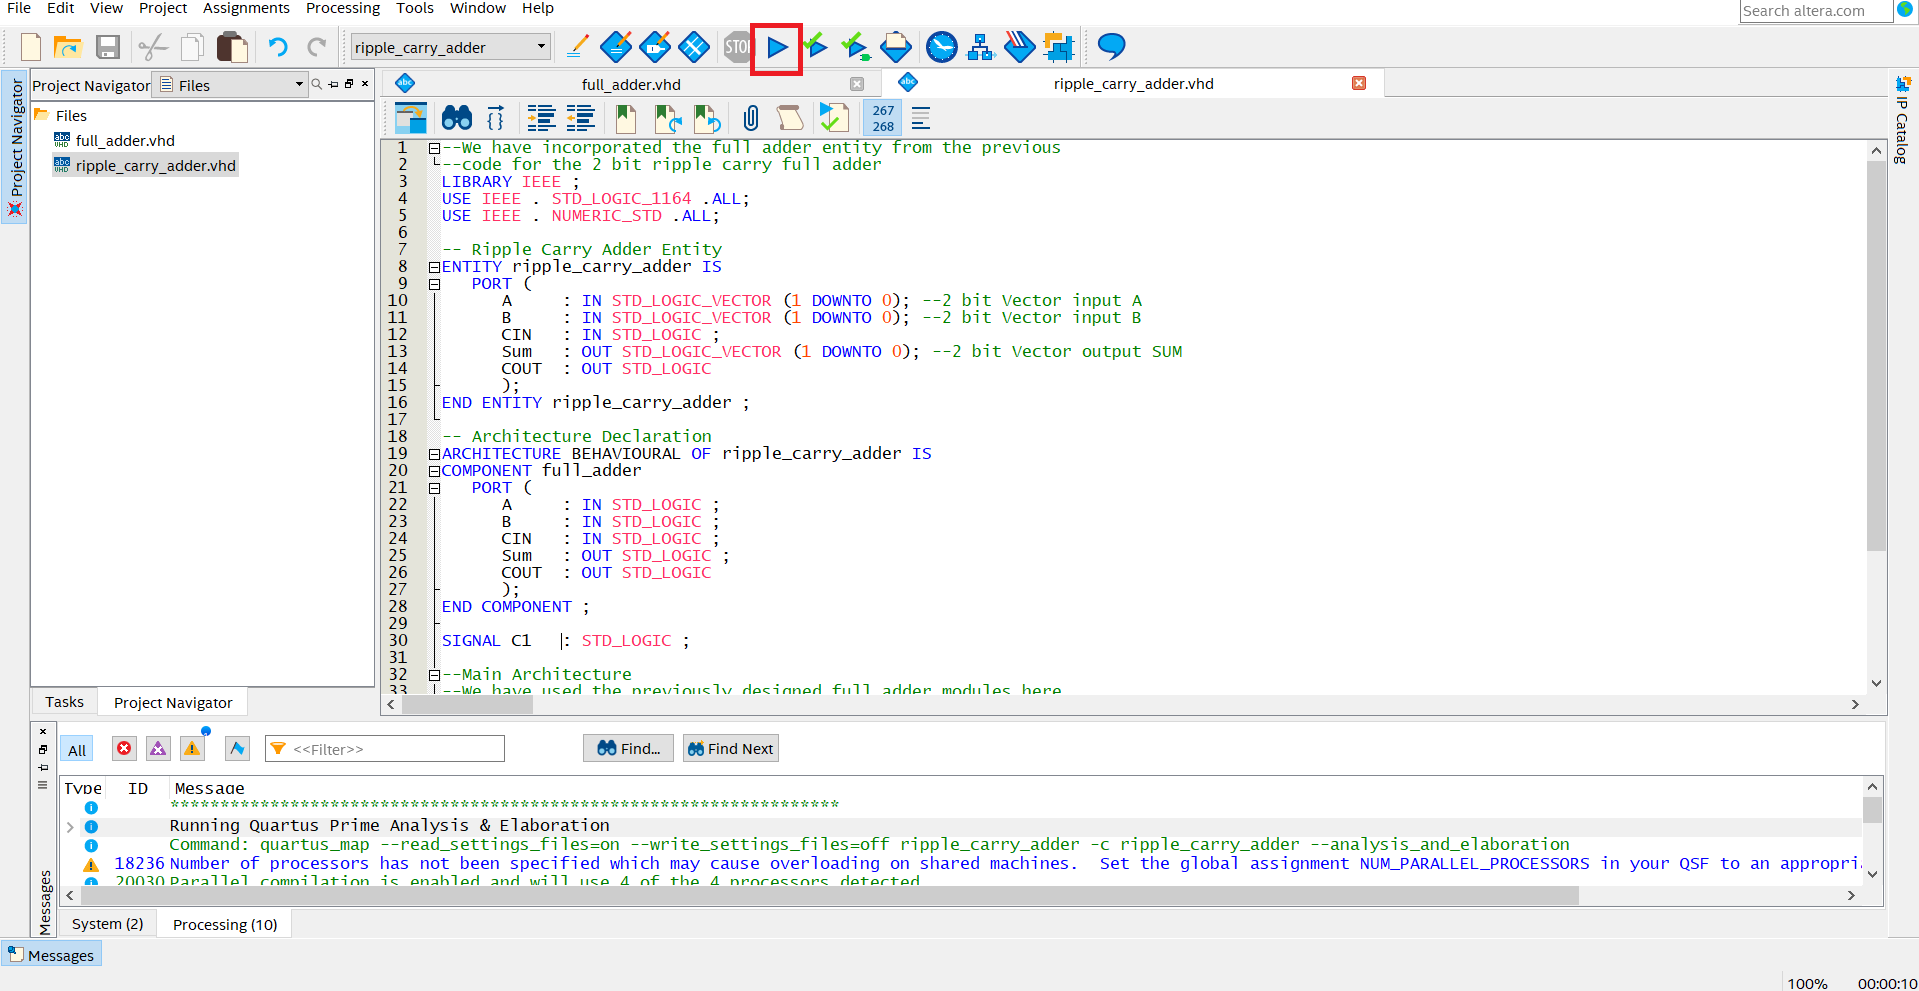
\includegraphics[width=14cm,keepaspectratio]{img16.png}
     \caption{Creating .SOF file}
     \end{figure}
     
     \item Open the programmer by going to \textbf{Tools}$\rightarrow$\textbf{Programmer}
     \begin{figure}[H]
         \centering
         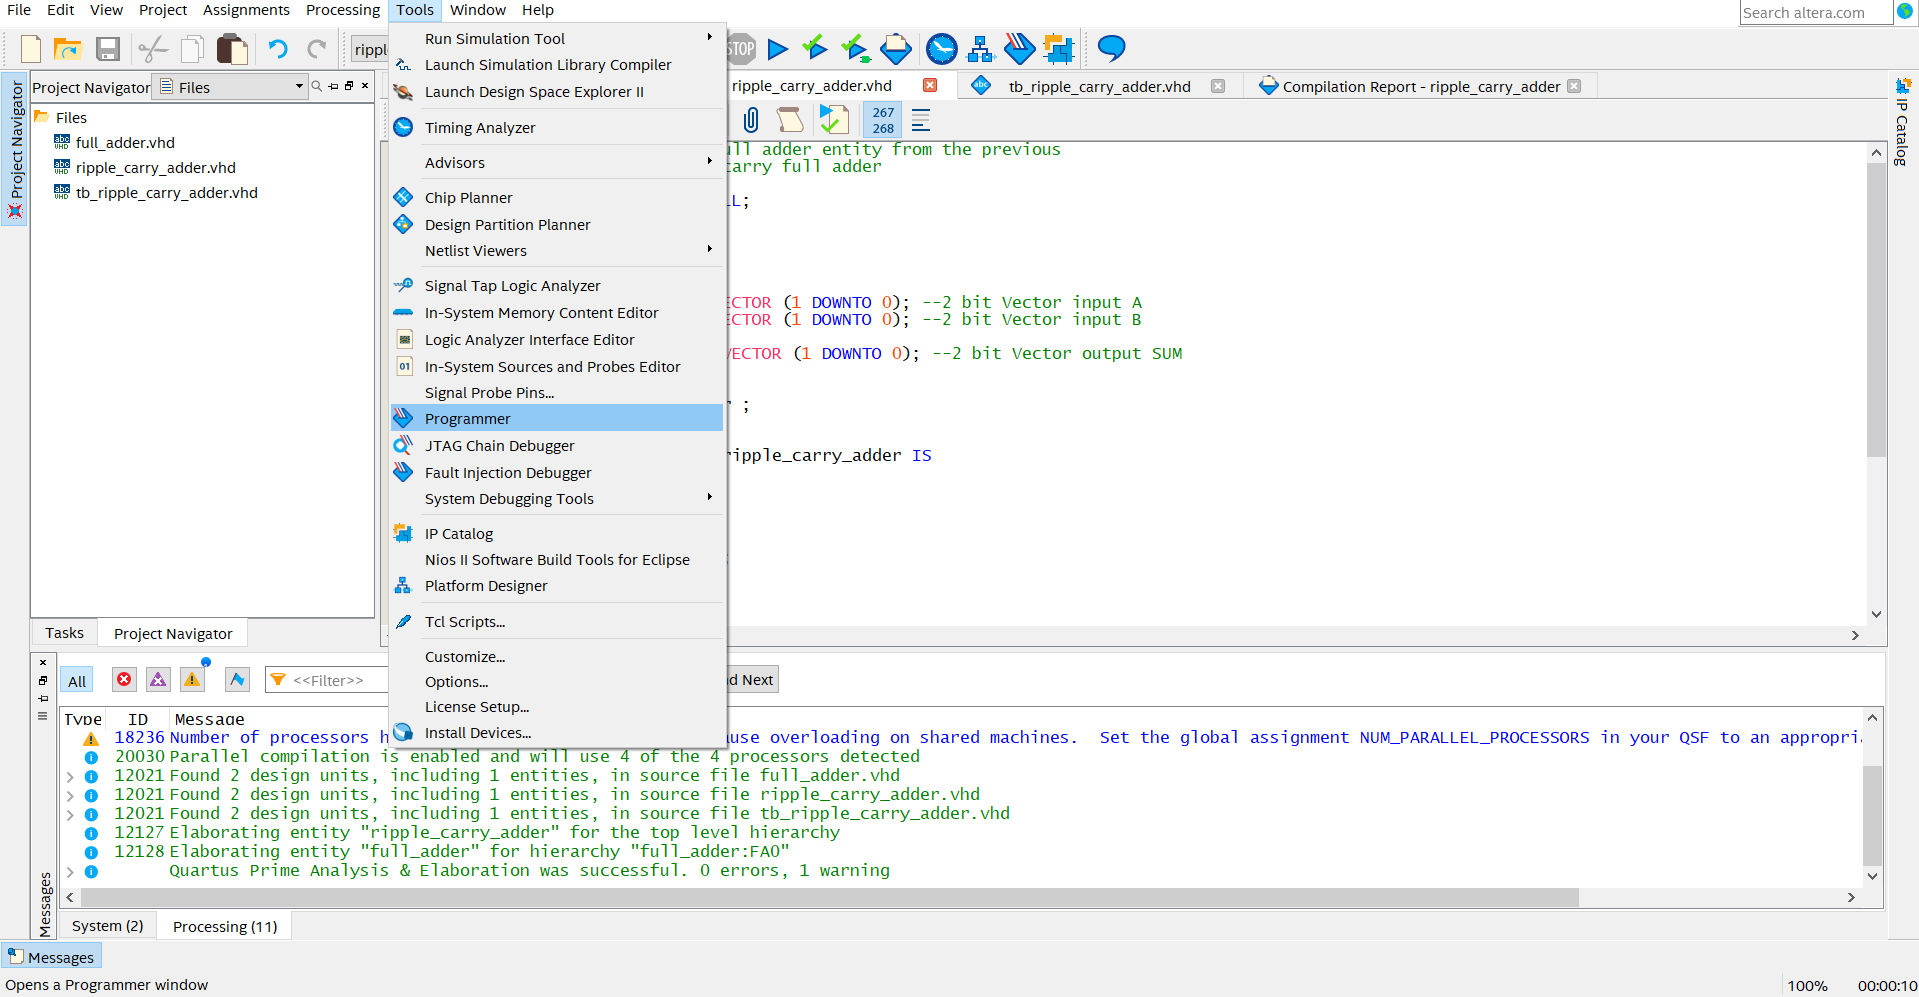
\includegraphics[width=14cm,keepaspectratio]{img17.png}
     \caption{Programmer}
     \end{figure}
     \newpage
     
     \item Click on \textbf{Hardware Setup}. The Device required must be listed under "Currently available hardware". If not, check if the device drivers are correctly installed. Choose the hardware from the dropdown menu
     \begin{figure}[H]
         \centering
         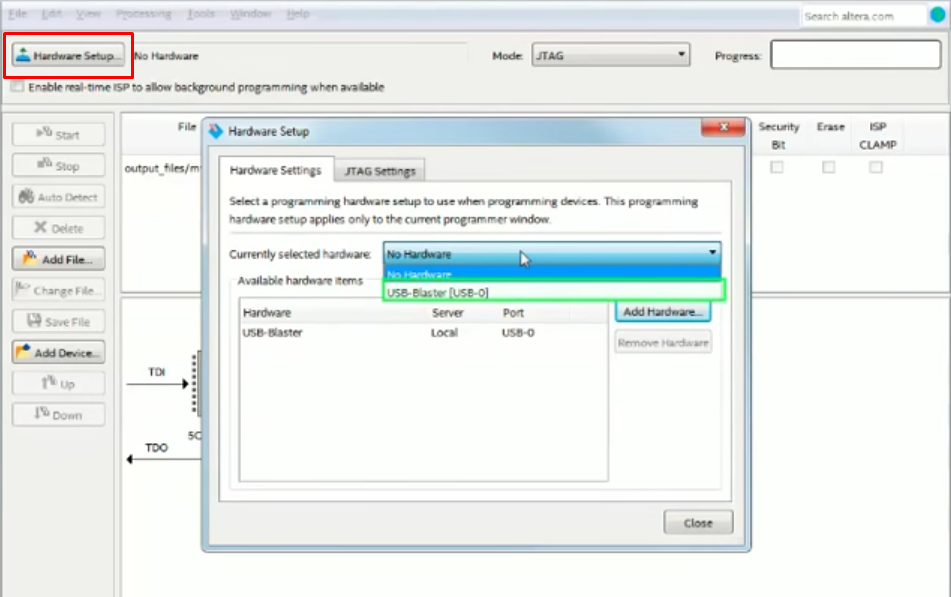
\includegraphics[width=14cm,keepaspectratio]{3.png}
     \caption{Hardware setup}
     \end{figure}
     
     \item If the file is not listed, it can be manually added by clicking on \textbf{Add File}. The .SOF file can be found the output directory inside the project directory 
     \begin{figure}[H]
         \centering
         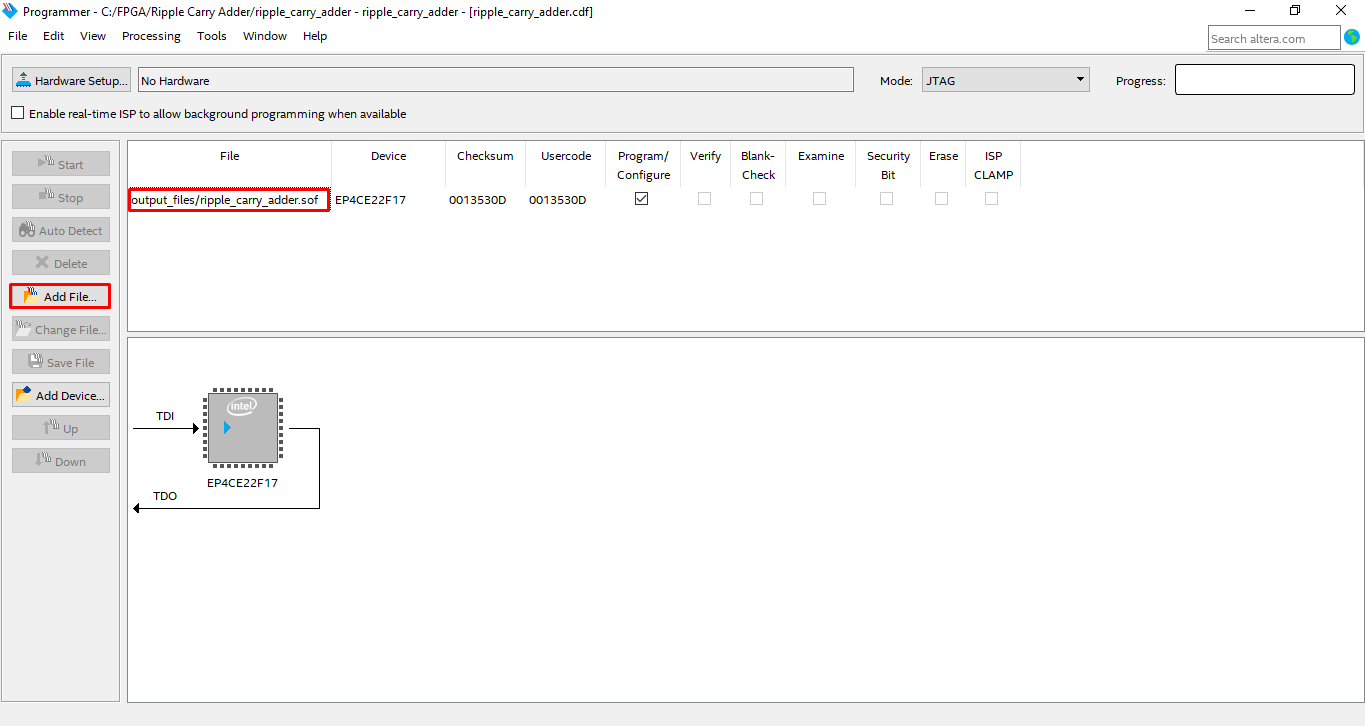
\includegraphics[width=14cm,keepaspectratio]{img19.png}
     \caption{Add file}
     \end{figure}
     \newpage
     \item Make sure the Program/Configure checkbox is ticked
     \begin{figure}[H]
         \centering
         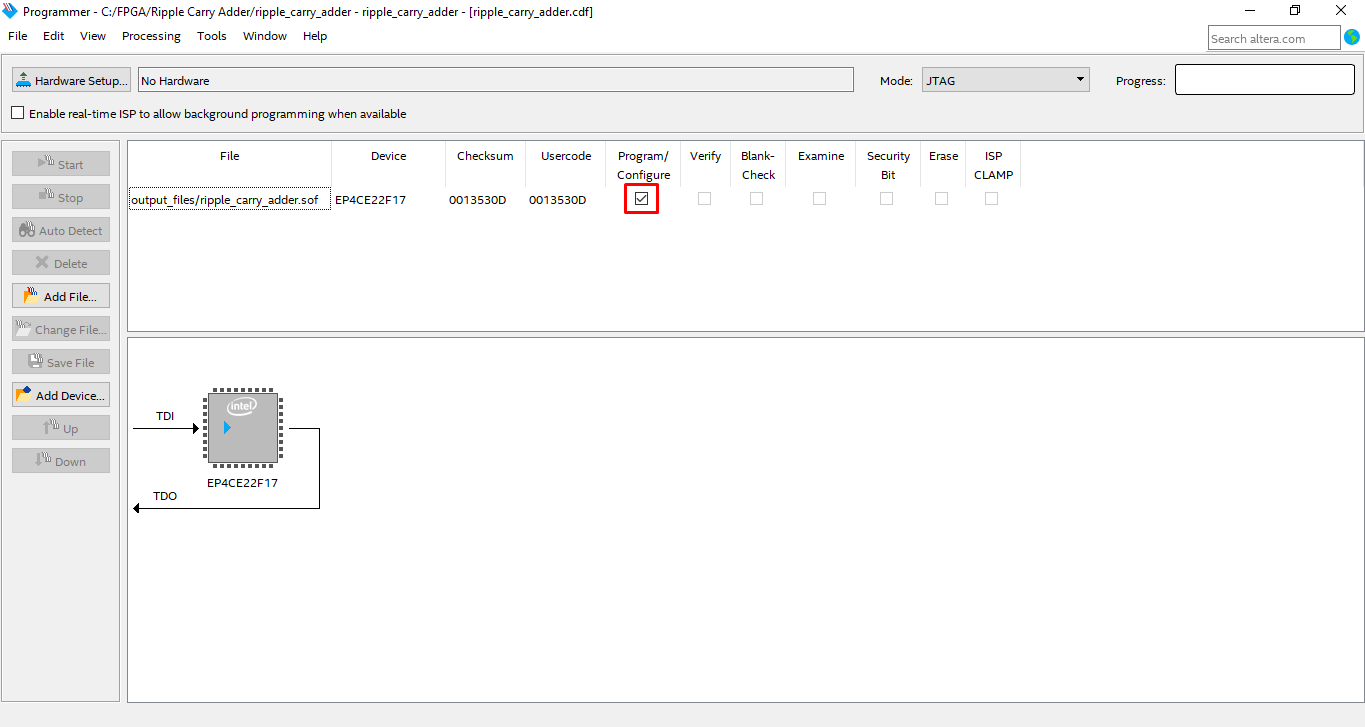
\includegraphics[width=14cm,keepaspectratio]{img20.png}
     \caption{Setting Program Configure}
     \end{figure}
     
     \item When ready, click on \textbf{Start} to start the programming process. \textbf{Start} button will be enabled when the 'DEO NANO' board is connected to USB port of your device. 
     \begin{figure}[H]
         \centering
         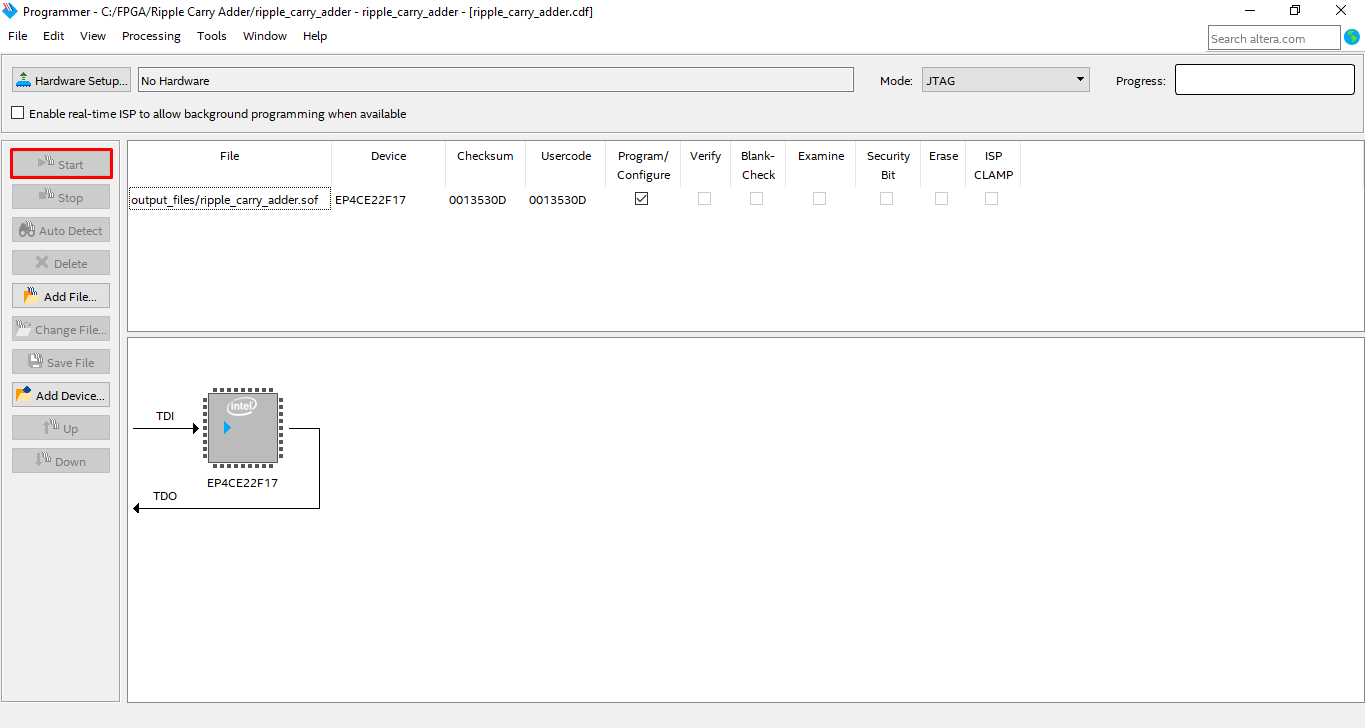
\includegraphics[height=7cm,keepaspectratio]{img21.png}
     \caption{Initiating Design Download into FPGA}
     \end{figure}
     
 \end{enumerate}
\newpage
\section{Implementing on Modelsim }
For more detailed procedure on using ModelSim, refer \textbf{Quick Start Guide to Quartus and ModelSim Software} Document. You can find both Verilog HDL and VHDL TestBench code below, make sure to follow only one language in this entire tutorial.

 \begin{enumerate}
     \item Create a New VHDL file in Quartus Prime.Type in the TestBench code provided in this document and save the file with the same name as the module name
    \begin{figure}[H]
        \centering
    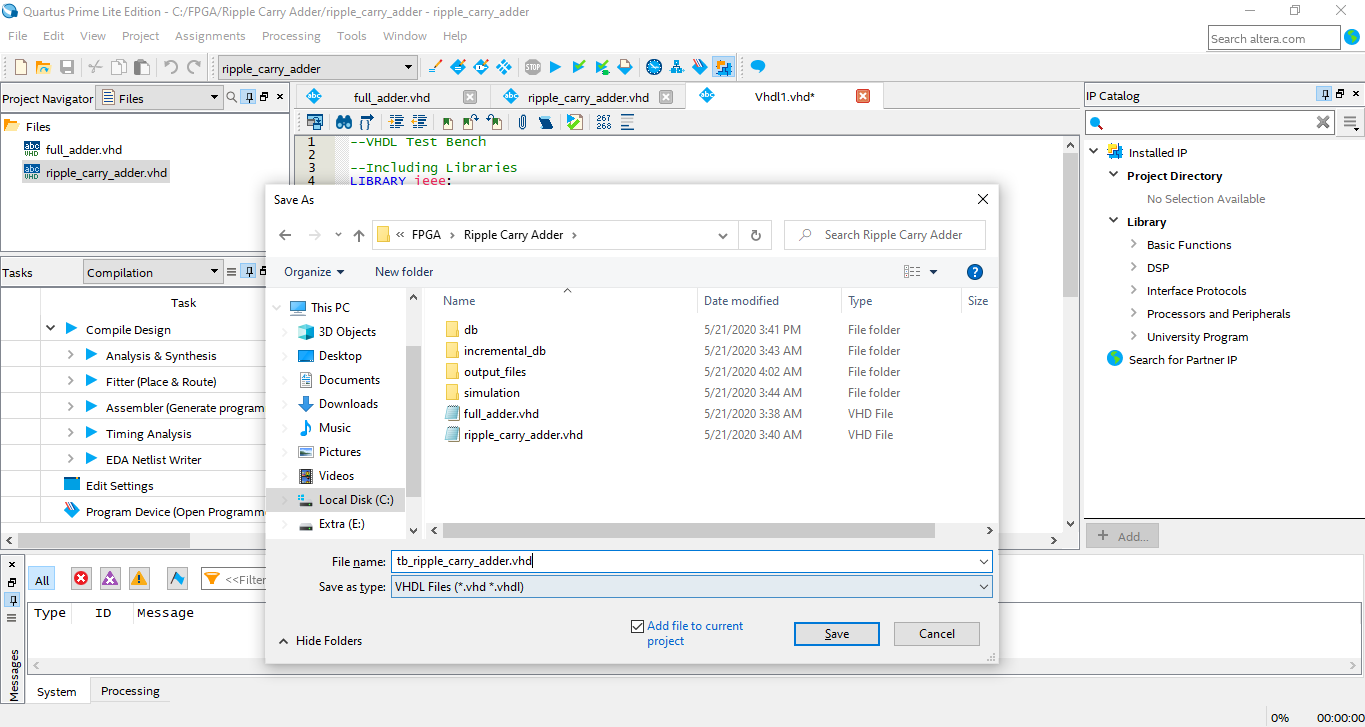
\includegraphics[width=14cm,keepaspectratio]{img22.png}
    \caption{Save TestBench file}
    \end{figure}
   
    \item Go to \textbf{Assignments}$\rightarrow$\textbf{Settings}.
    \begin{figure}[H]
        \centering
    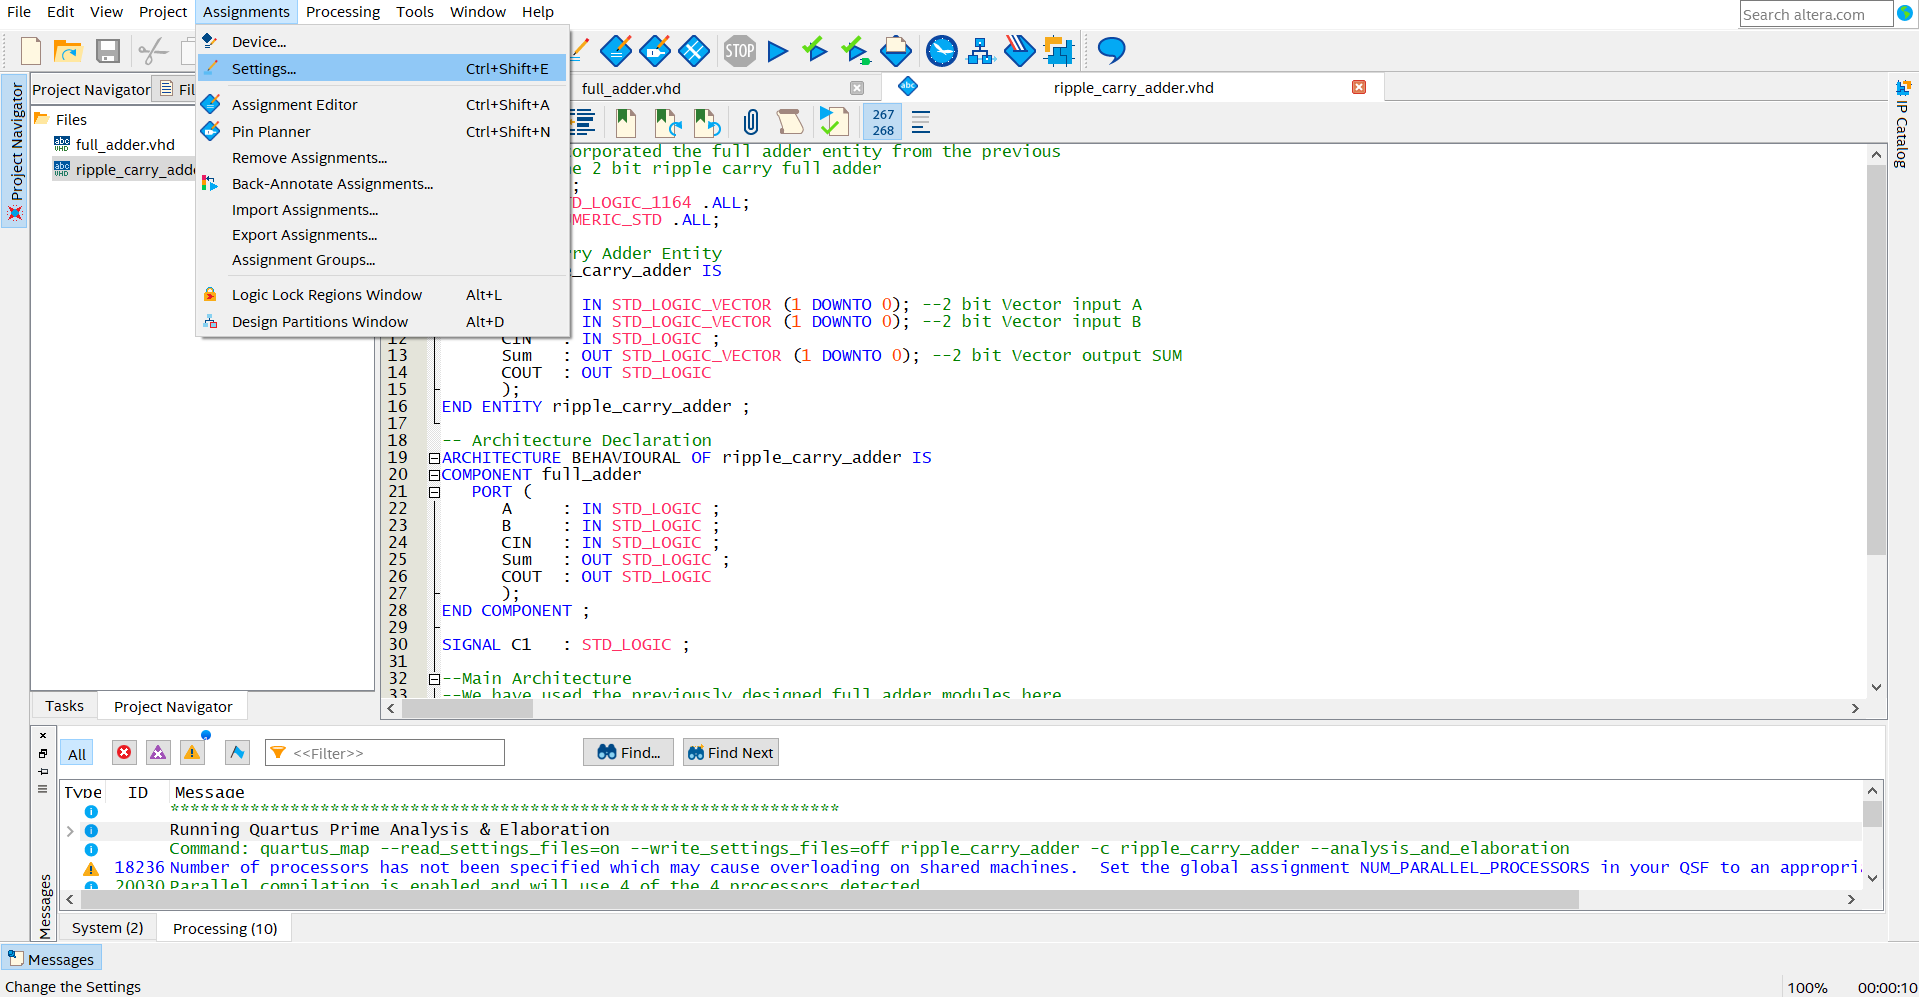
\includegraphics[width=14cm,keepaspectratio]{img23.png}
    \caption{Settings}
    \end{figure}
    \newpage
    \item Navigate to \textbf{Simulation} under \textbf{EDA Tool Settings}.Set the language as VHDL. Select \textbf{Compile TestBench} and then click on \textbf{Test Benches}.
    \begin{figure}[H]
        \centering
    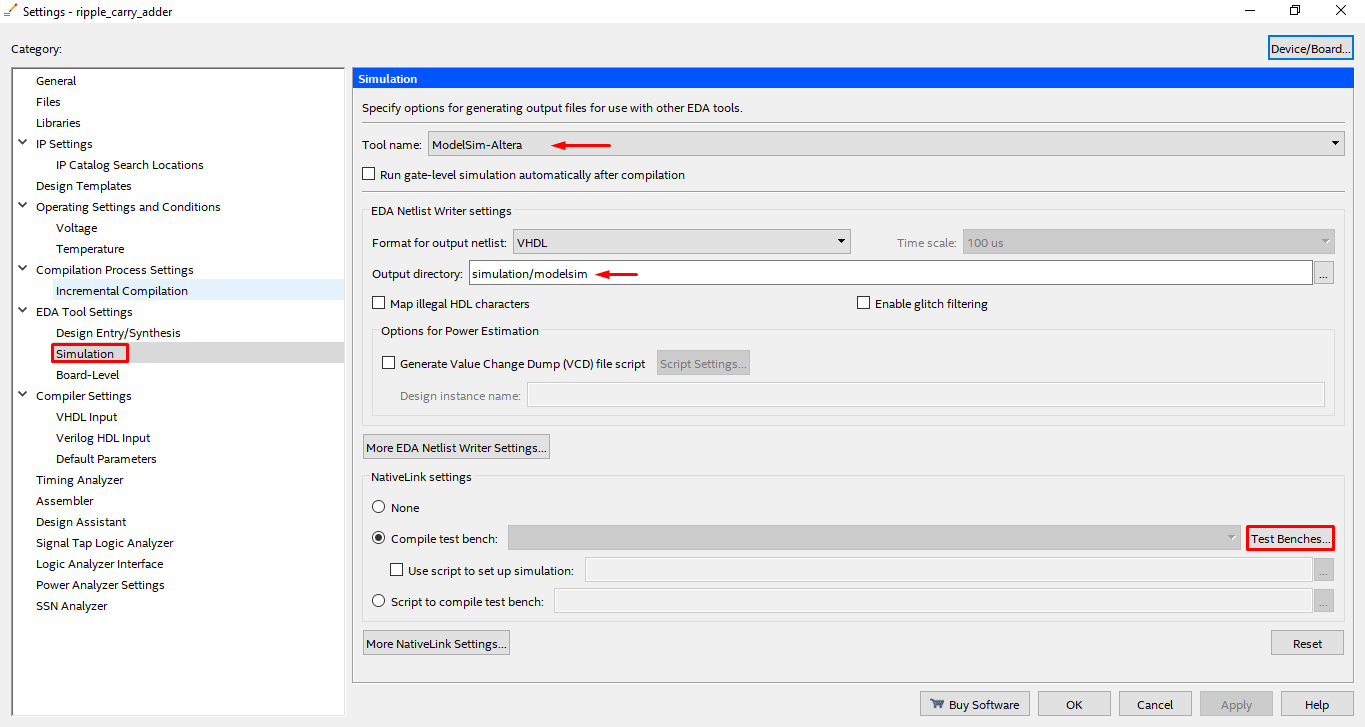
\includegraphics[width=14cm,keepaspectratio]{img24.png}
    \caption{Adding the TestBench file}
    \end{figure}
  
    \item Click on \textbf{New}, this opens another dialogue box.
    \begin{figure}[H]
        \centering
    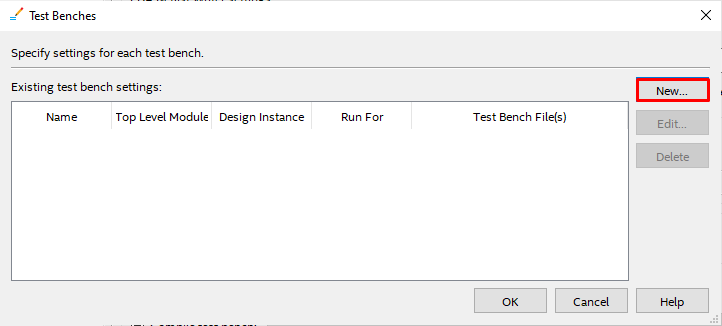
\includegraphics[width=14cm,keepaspectratio]{img25.png}
    \caption{Adding the TestBench file}
    \end{figure}
    \newpage
    \item Now type in the TestBench name(In this design , its \textbf{tb\_ripple\_carry\_adder}). Now click on the highlighted Browse button.Find the TestBench file(it can be found in the project directory) and click on \textbf{Open}. Now click on \textbf{Add},then \textbf{OK}.
            \begin{figure}[H]
        \centering
    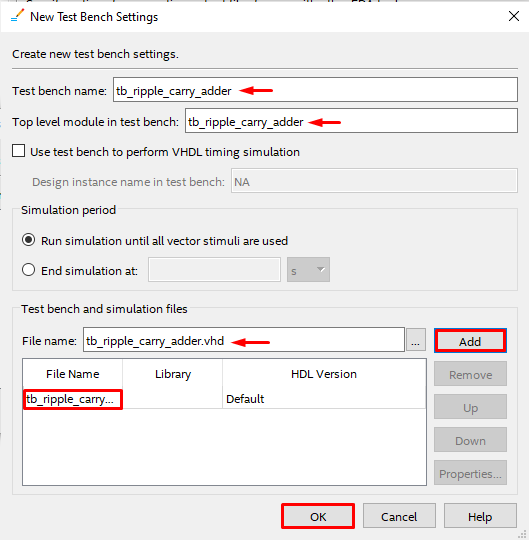
\includegraphics[scale=0.73]{img26.png}
    \caption{Adding the TestBench file}
    \end{figure}
    
 \end{enumerate}

 \noindent \textbf{Functional Simulation using NativeLink Feature}
    \begin{enumerate}
        
        \item  Go to \textbf{Processing}$\rightarrow$\textbf{Start Compilation}
            \begin{figure}[H]
                \centering
                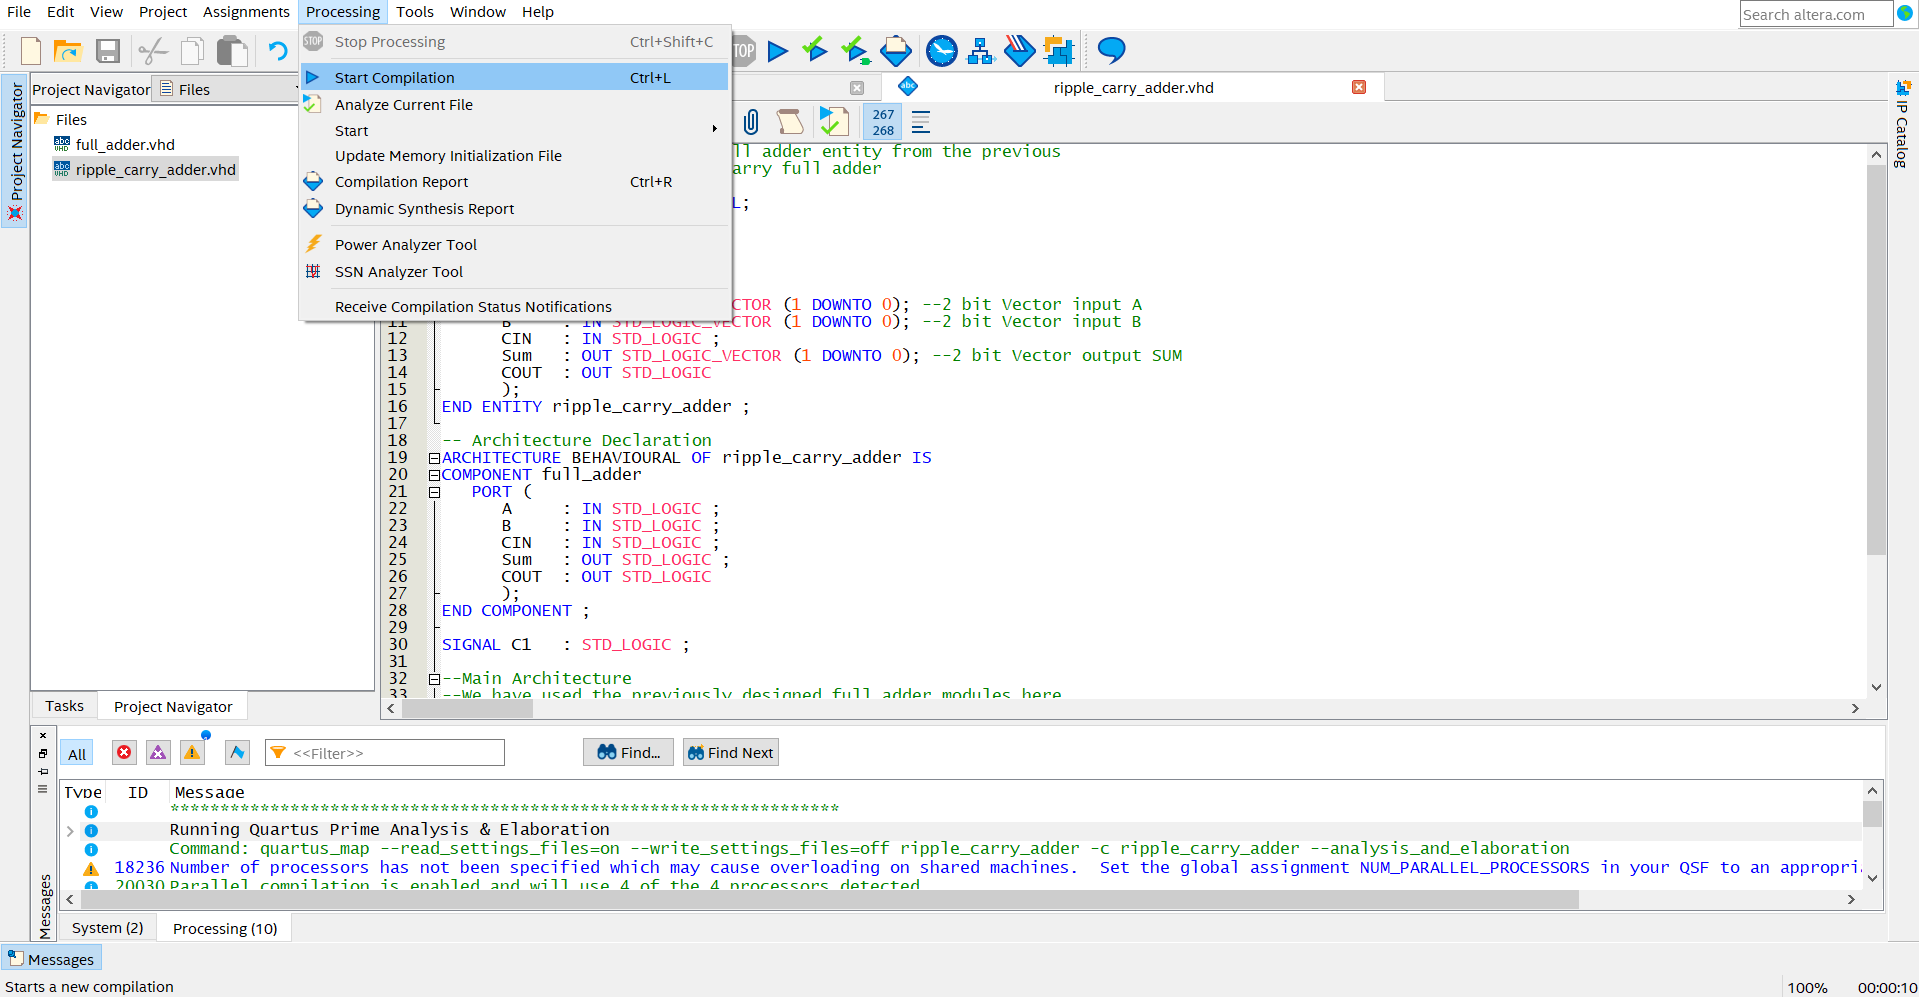
\includegraphics[width=14cm,keepaspectratio]{img7.png}
            \caption{Compiling the project}
            \end{figure}
    
        \newpage
        \item Go to \textbf{Tools}$\rightarrow$\textbf{Run Simulation Tool}$\rightarrow$\textbf{RTL Simulation} to automatically run the EDA simulator(ModelSim-Altera) and to compile all necessary design files.
            \begin{figure}[H]
                \centering
                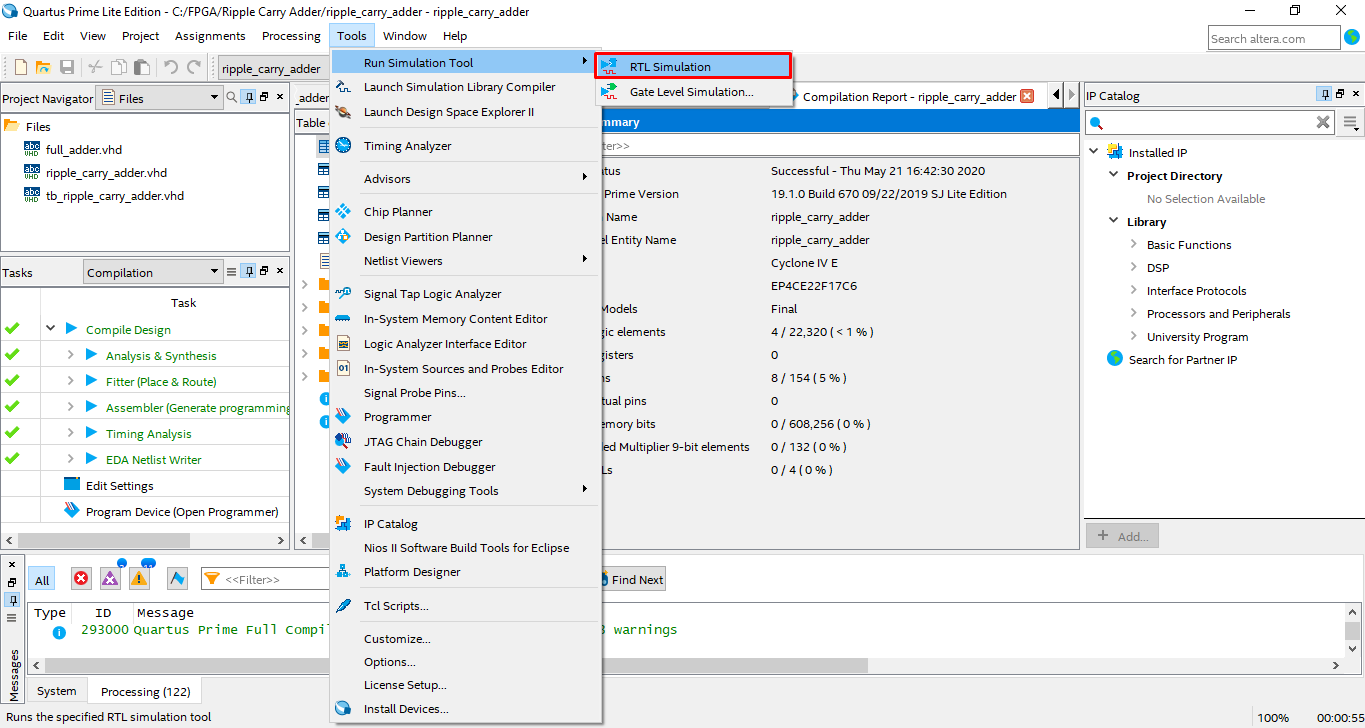
\includegraphics[width=14cm,keepaspectratio]{img28.png}
            \caption{RTL Simulation}
            \end{figure}

        \item Finally ModelSim-Altera tool opens up with simulated waveform. click on \textbf{Run all} icon on the tool box to display the waveform.\textbf{Note:} If you cannot see the waveform, Click on the waveform window and select the \textbf{Zoom all} option.
            \begin{figure}[H]
                \centering
                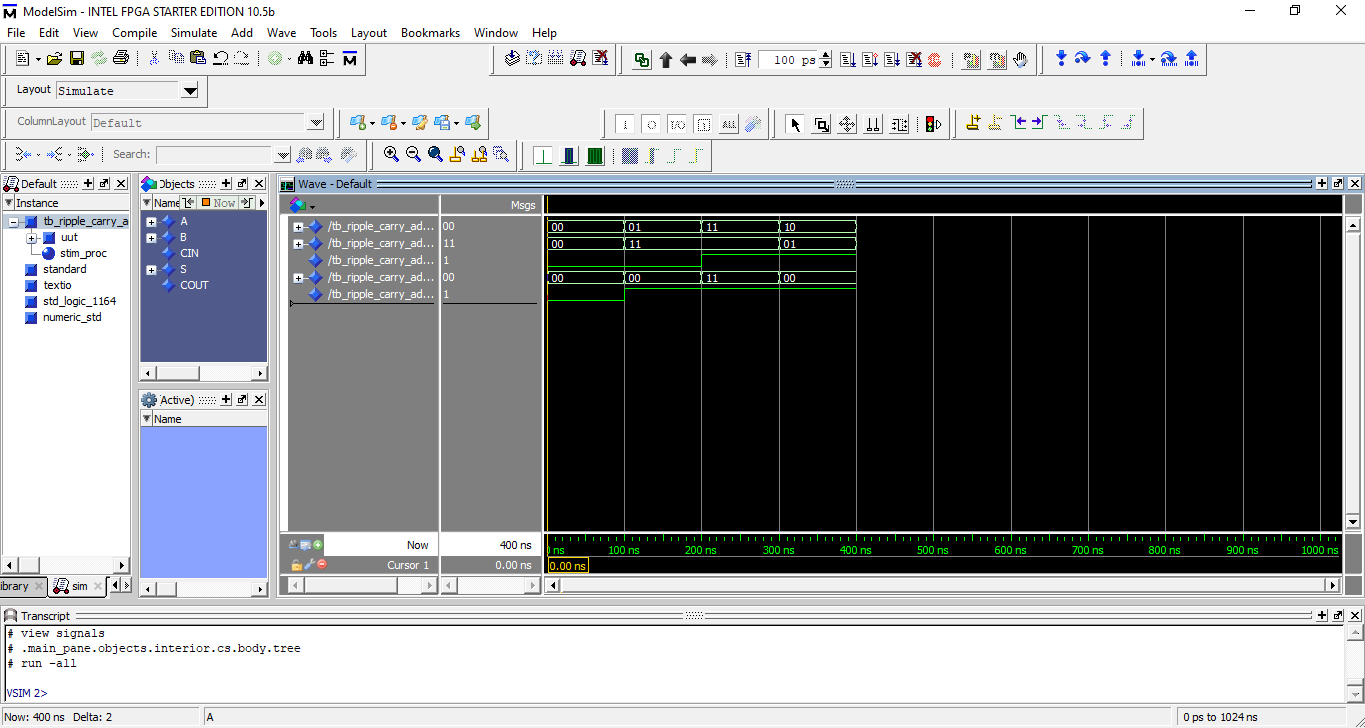
\includegraphics[width=14cm,keepaspectratio]{img29.png}
            \caption{RTL Simulation}
            \end{figure}
        
    \end{enumerate}
\newpage
\section{Testing the Design}

\subsection{Simulation waveform of the VHDL Design}
The Result shown below can be verified by comparing it with the Truth Table provided in page 2
You can observe individual bits of a particular signal by clicking on the '+' icon.
\begin{figure}[H]
    \centering
    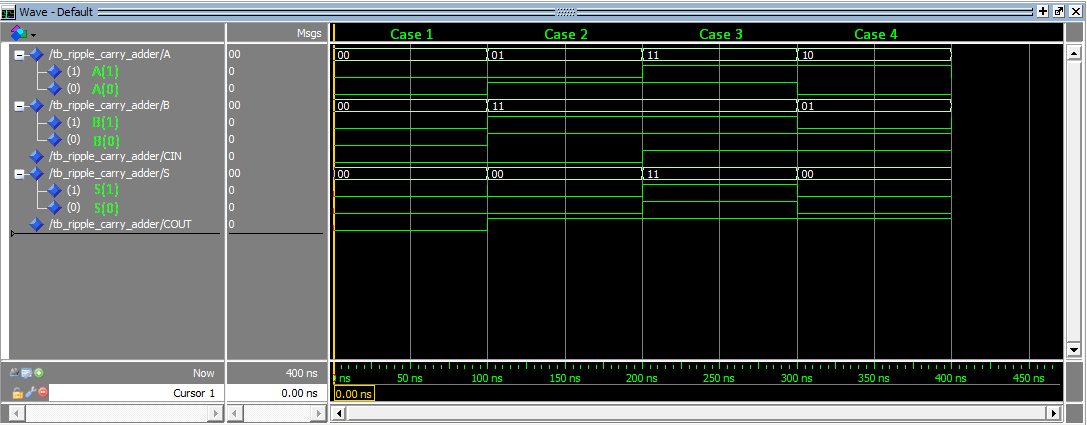
\includegraphics[width = 14cm,keepaspectratio]{img30.png}
\caption{Simulation waveform}
\end{figure}

\end{document} 
 
